\documentclass[review,12pt]{elsarticle}


\usepackage[utf8]{inputenc}
\usepackage[T1]{fontenc}
\usepackage{lmodern}
\usepackage{amsmath,amssymb,amsfonts,mathtools}
\usepackage{url}
\usepackage{graphicx}
\usepackage{booktabs}
\usepackage{multirow}
\usepackage{array}
\usepackage{float}
\usepackage{placeins}
\usepackage{setspace}
\usepackage{xcolor}
\usepackage{caption}
\usepackage{subcaption}
\usepackage{enumitem}
\usepackage{tabularx}
\usepackage{rotating}
\usepackage{adjustbox}
\usepackage{makecell}
\newcolumntype{Y}{>{\raggedright\arraybackslash}X}
\usepackage{tikz}
\usetikzlibrary{arrows.meta,positioning,calc,decorations.pathreplacing}
\usepackage{helvet} 
\usepackage{amsthm}
\newtheorem{proposition}{Proposition}
\usepackage[colorlinks=true,linkcolor=blue,citecolor=blue,urlcolor=blue]{hyperref}
\pdfstringdefDisableCommands{%
  \def\corref#1{}%
  \def\cortext#1#2{}%
  \def\ead#1{}%
}


\setlength{\parindent}{1.5em}
\setlength{\parskip}{0pt}

\onehalfspacing
\setlength{\emergencystretch}{2em}

\newcolumntype{L}[1]{>{\raggedright\arraybackslash}p{#1}}
\newcolumntype{C}[1]{>{\centering\arraybackslash}p{#1}}
\renewcommand{\arraystretch}{1.15}

\journal{Transportation Research Part C: Emerging Technologies}

\begin{document}

\hypersetup{pageanchor=false}
\begin{frontmatter}

\title{A Dynamic Coordination Horizon Framework for Traffic Signal Control: Diagnosing Controller Effectiveness Across Operating Regimes}

\author[inst1]{Mohamed Yassine Neifar\corref{cor1}}
\ead{yessine.neifar.imsil@isgis.usf.tn}
\cortext[cor1]{Corresponding author.}
\author[inst1]{Nadir Farhi}
\author[inst2]{Ahmed Frikha}
\address[inst1]{Universit\'e Gustave Eiffel, COSYS--GRETTIA,
14--20 Boulevard Newton, Cit\'e Descartes, Champs-sur-Marne,
F-77447 Marne-la-Vall\'ee Cedex 2, France}

\address[inst2]{Institut Sup\'erieur de Gestion Industrielle de Sfax,
OLID, University of Sfax, Route de l'A\'eroport km 4, BP 1099,
Sfax 3038, Tunisia}

\begin{abstract}
Cooperative traffic signal control is increasingly studied with
multi-agent reinforcement learning (MARL), yet evaluations rarely
identify where coordination opportunities exist, where a fixed policy
generalizes, or which controller family performs best. This paper
proposes a Dynamic Coordination Horizon Framework (DCHF) that diagnoses
benchmark-relative approximation, capacity pressure, and controller-family
suitability across spacing, demand, and network size. It is implemented
in SUMO--TraCI using QMIX, an optimized fixed-offset benchmark, and a
non-learning Max Pressure reference.

Max Pressure gives the
lowest waiting measure at the tested 100, 200, and 300~m spacings. At
500~m the optimized offset is strongest and retains a material
progression opportunity; at 750 and 1000~m the best swept plan provides
essentially no improvement over simultaneous fixed-time control,
indicating collapse of that opportunity. At $d=300$~m, Max Pressure is
best at all five demand levels. In the ten-seed reference corridor,
QMIX~V2 remains within $4.42\%$ of the optimized offset, although Max
Pressure performs best. The spatial and demand experiments characterize
fixed-policy generalization without retraining. After paired multi-seed evidence is
incorporated for 15 cells, the exploratory 30-cell distance--demand grid
contains three usefully effective, three capacity-constrained, four
marginal, and twenty outside-horizon conditions. A five-intersection
stress test finds effectiveness in only three of sixteen exploratory
conditions.

The DCHF identifies where a fixed-offset coordination opportunity
exists, where a fixed learned policy generalizes, and how the
best-performing tested family changes along the directly evaluated
spatial and demand slices.
\end{abstract}
\begin{keyword}
Traffic signal coordination \sep Coordination horizon \sep Multi-Agent Reinforcement Learning \sep QMIX \sep Max Pressure \sep SUMO--TraCI
\end{keyword}

\end{frontmatter}
\hypersetup{pageanchor=true}


\section{Introduction}
\label{sec:introduction}

Urban congestion produces excessive delay, queue formation, unreliable travel times, and emissions, driven in part by insufficient signal coordination~\cite{rahman2022,balaci2024}. Signal control is central to traffic management because timing decisions shape progression, queue dissipation, intersection capacity, and corridor stability~\cite{hale2002}. Traditional fixed-time, actuated, and offset-based strategies remain widely used for their simplicity and low cost; classical coordination relies on progression, cycle length, offsets, platoon dispersion, and bandwidth maximization~\cite{paoloserafini1989,jingquanli2014,farzaneh2006}. A well-tuned offset plan already captures much of the available corridor benefit, making it a demanding benchmark for any learning-based controller.

Reinforcement learning (RL) and multi-agent reinforcement learning (MARL) have emerged as adaptive alternatives. For isolated intersections, deep RL methods such as Deep Q-Networks adapt signal decisions to changing conditions~\cite{Mnih2015,jamil2024}. Real corridors, however, comprise interacting intersections, where a decision at one junction affects downstream queues, upstream spillback, and corridor throughput, making coordination a natural multi-agent problem. Among cooperative MARL methods, QMIX is relevant because it supports centralized training with decentralized execution~\cite{Rashid2018}: training exploits global state while execution uses only local observations, matching the asymmetry between simulation-based training and intersection-local deployment.

Despite this progress, a central question remains insufficiently addressed: when does cooperative coordination actually help? Network-level RL traffic-signal studies commonly use fixed-time, actuated, or other non-optimized baselines, so reported gains often show improvement over the selected reference rather than proximity to a strong coordination-oriented benchmark~\cite{noaeen2022reinforcement}. Recent MARL studies illustrate this evaluation pattern~\cite{zhang2022distributed,hu2024,jia2025multi,shang2025graph}. Yet coordination is not automatically beneficial; its value depends on corridor geometry, interaction strength, demand, storage capacity, and network size, so a policy effective in one region can fail in another. Five limitations are rarely characterized together: (i)~the \emph{spatial} limit, determining how far upstream information remains useful before platoon dispersion erodes it; (ii)~the \emph{demand} limit, with weak interaction under sparse demand and capacity pressure under heavy demand; (iii)~the \emph{capacity and spillback} limit, under which storage constraints can be misread as controller failure; (iv)~the \emph{scalability} limit, concerning whether coordination persists as the network grows; and (v)~the use of \emph{weak classical baselines}, which can exaggerate learning gains when an optimized fixed-offset plan already captures most of the coordination benefit.

This paper reframes cooperative signal control as the problem of identifying the \textit{limits of useful coordination}. The main contribution is not the use of QMIX but a \textbf{Dynamic Coordination Horizon Framework} (DCHF) that diagnoses coordination usefulness over controlled spacing, demand, and network size while also reporting the controller-specific capacity state. Each condition is classified as effective, marginal, capacity-constrained, or outside the useful horizon through the spatial $H_S$, demand $H_D$, capacity $H_B$, and scalability $H_N$ diagnostics. QMIX serves only as the cooperative MARL instrument that populates this diagnosis. The DCHF is algorithm-independent as a protocol---the benchmark-relative gap can be computed for any controller---but the empirical horizons reported here are controller-conditional: they characterize the tested QMIX~V2 implementation, the binary action space, the SUMO corridor design, and the evaluated demand regimes, and should not be read as universal limits of cooperative MARL.

The DCHF combines two indicators with a deliberate hierarchy: Coordination Gain as a supporting measure relative to uncoordinated simultaneous fixed-time control, and the MARL approximation gap, as the primary diagnostic, measuring how closely a learned policy approaches an optimized fixed-offset benchmark obtained by exhaustive sweep. Measuring distance from a strong benchmark, rather than improvement over a weak one, distinguishes genuine coordination quality from algorithmic approximation error or capacity-constrained performance. A buffered-ratio diagnosis distinguishes approximation limits from controller-specific insertion-capacity pressure, while a strong acyclic Max Pressure controller provides a non-learning adaptive reference.

The main contributions are as follows.
\begin{itemize}
\item A \textbf{Dynamic Coordination Horizon Framework} (DCHF) that classifies each condition as effective, marginal, capacity-constrained, or outside the useful horizon along the spatial $H_S$, demand $H_D$, capacity $H_B$, and scalability $H_N$ horizons, built on the \textbf{MARL approximation gap} as its primary measure with \textbf{Coordination Gain} and the buffered ratio as supporting diagnostics.

\item A \textbf{controller-family diagnostic interpretation}. In the unconstrained two-intersection Scenario~A reference corridor, Max Pressure obtains the best performance ($149.911 \pm 2.640$~s, Wilcoxon signed-rank, $n=10$, $p=0.001953$), while QMIX~V2 remains close to the optimized fixed-offset benchmark (gap $4.42\%$, Wilcoxon signed-rank, $n=10$, $p=0.001953$). This supports the diagnostic role of the DCHF: different controller families may be appropriate in different operating regimes.

\item A progressive SUMO--TraCI experimental design with ten-seed formal statistical validation in the Scenario~A reference and the Scenario~B transfer, and five-seed bootstrap validation at the boundary-defining spatial and demand conditions, with single-seed mapping retained for the remaining interior cells of the joint distance--demand grid. All reported seeds are evaluation seeds applied to fixed trained policies, not independent training runs.

\item \textbf{Preliminary scalability observation.}\newline The strongest $N=5$ evidence is the five-seed homogeneous $d=300$~m, medium-demand reference condition, evaluated against a one-parameter cumulative progression-offset benchmark. In the separate single-seed 16-cell $N=5$ distance--demand stress grid, only three point estimates are effective, and the two long-spacing cases do not establish a contiguous effective region (Section~\ref{subsec:n5_distance_demand_stress}). Scalability therefore remains conditional, and its upper network-size boundary is not located.
\end{itemize}

\textbf{Problem statement and research questions.} For an arterial corridor of $N$ signalized intersections, the objective is not only to minimize the network-level waiting measure but to identify the operating conditions under which coordination is useful, in the regime sense formalized in Section~\ref{subsubsec:coordination_regime}. Four research questions structure the experimental design:

\begin{enumerate}[label=\textbf{RQ\arabic*.}, leftmargin=1.5cm]
\item How can useful traffic signal coordination be diagnosed beyond 
average performance improvement, by combining Coordination Gain, the 
MARL approximation gap, and a capacity diagnosis?
\item How do inter-intersection spacing and demand, together with observed
controller-specific capacity pressure, shape the spatial, demand, and
capacity diagnostics $\{H_S,H_D,H_B\}$?
\item How does coordination usefulness evolve as the number of controlled 
intersections increases, defining the scalability horizon $H_N$?
\item Can cooperative MARL approximate optimized classical coordination 
within effective regimes, and how does it compare with a strong Max 
Pressure baseline?
\end{enumerate}

The cooperative MARL formulation and standard learning equations are provided in Supplementary Section~S-8; Supplementary Sections~S-1 to S-11 collect the threshold derivation, configurations, single-seed exploratory maps, and extended validation tables referenced throughout.


\section{Literature Review}
\label{sec:literature}

\subsection{Classical coordination}
\label{subsec:lit_classical}

Classical arterial coordination rests on a common cycle, green-split allocation, offset optimization, and progression-bandwidth maximization. Robertson's TRANSYT established that a well-calibrated fixed-offset plan minimizes corridor delay by coordinating platoon arrivals~\cite{robertson1969transyt}; MAXBAND~\cite{jingquanli2014,little1981maxband} and MULTIBAND~\cite{gartner1990multiband} extended this to globally optimal bandwidth solutions concentrating green windows around predicted platoon positions, and PASSER generalized bandwidth methods to mixed phasing and diverse topologies~\cite{binbinjing2023}. The implication for learning-based evaluation is direct: a well-tuned fixed-offset plan already captures a large share of the corridor benefit, even under progression-time uncertainty~\cite{sangkeykim2015} and in oversaturated regimes~\cite{monttygirianna2004,xiaolongma2020}. Simultaneous fixed-time control (zero or arbitrary offsets) is therefore a weak baseline whose lack of adaptivity motivates learning-based control. The present work accordingly uses a swept optimized-offset plan as its primary reference for the approximation gap~$G$, anchoring DCHF classifications to a competitive rather than naive baseline.

\subsection{Adaptive and actuated control}
\label{subsec:lit_adaptive}

Actuated control adjusts green at each intersection from detector data, and adaptive systems such as SCOOT~\cite{hunt1981traffic} and SCATS~\cite{sims1980scoot} extend this to incremental network-level adjustment of cycles, splits, and offsets; their reported delay margin over fixed-time control narrows once the fixed-time plan is itself well optimized~\cite{cameronkergaye2010}.

Max Pressure warrants separate treatment as a primary baseline. Under its
stated network and demand assumptions, the canonical controller has a
maximum-stability property for feasible demand and determines signal
actions from locally available queue information~\cite{varaiya2013max}.
That result concerns queue stability and throughput feasibility rather
than direct minimization of delay or arterial progression: the base
formulation is acyclic and myopic, and the pressure objective neither
optimizes corridor offsets nor targets platoon travel times. Practical
phase-service constraints further separate the theoretical controller
from an operational implementation, since cyclical variants require a
modified formulation and a corresponding stability analysis, and the
added phase-structure constraints can themselves affect operational
performance~\cite{levin2020max}. Progression-aware extensions exist---
C-MP, for example, incorporates platoon-sensitive information to improve
arterial coordination while retaining a maximum-stability property under
its stated assumptions~\cite{ahmed2025cmp}---but the present study
deliberately retains the standard acyclic formulation, which neither
detects moving platoons nor optimizes a corridor progression pattern, as
a transparent non-learning diagnostic reference. Its myopia reflects a
limitation shared by many locally adaptive methods~\cite{mikesmith2011},
which is the entry point for cooperative multi-agent learning.

\subsection{Reinforcement learning at isolated intersections}
\label{subsec:lit_rl_isolated}

Deep RL replaces the explicit traffic model with a learned state--action mapping, from tabular Q-learning~\cite{samaheltantawy2014} through DQN-based models at single intersections~\cite{sangminpark2021,mohammadaslani2018} to later refinements of state representation, architecture, and reward design~\cite{wei2018intellilight,wei2019presslight,chen2020toward}. By construction, an isolated agent sees no upstream or downstream state and cannot tell whether coordination would help; benchmarked against optimized rather than weak fixed-time control, the reported margin of isolated RL can narrow or disappear~\cite{chenouyang2024}; benchmark sensitivity also remains relevant in network-level RL studies~\cite{noaeen2022reinforcement}.
\subsection{Multi-agent reinforcement learning for traffic networks}
\label{subsec:lit_marl}

In MARL formulations each intersection is an agent optimizing a network reward, spanning independent learning, centralized training with decentralized execution (CTDE), centralized-critic actor--critic methods~\cite{yu2022surprising}, and graph- and communication-based designs~\cite{analcbazzan2008,ammarhaydari2022,noaeen2022reinforcement}. CTDE methods reduce corridor delay beyond fixed-offset control~\cite{zhang2022distributed}, graph- and attention-based controllers increasingly learn \emph{which} neighbours matter~\cite{taowang2024,chengdongma2024}, and curriculum and network-wide variants have proliferated~\cite{xuesili2023,fuyueren2023,jiefang2023}. This shift---toward how far upstream information should travel and which neighbours to weight---implicitly treats coordination value as neighbour- and distance-dependent, the premise the spatial horizon makes explicit and measurable.

Benchmark selection remains heterogeneous across network-level studies of reinforcement-learning traffic signal control, with fixed-time and other non-optimized references commonly used in the reviewed literature~\cite{noaeen2022reinforcement}. Such comparisons demonstrate adaptivity but conflate the quality of the learned controller with the weakness of the selected reference; the present study addresses this ambiguity by using an exhaustively swept optimized fixed-offset plan as the primary approximation benchmark. A more fundamental gap persists: the conditions under which coordination is beneficial have received little systematic empirical attention. Studies from foundational large-scale architectures~\cite{chu2019multi} to recent attention-based and multi-objective variants~\cite{andechang2024,jia2025multi,nie2025cmrm,huang2026robust} improve performance under specific configurations but give limited evidence on where coordination gains diminish or how effectiveness evolves with spacing, demand, network size, and congestion.

The closest conceptual precursor to the coordination-horizon idea is the spatial discount factor of Chu et al.~\cite{chu2019multi}, which attenuates the reward contribution of distant agents and thereby encodes the assumption that coordination matters less with distance. That mechanism, however, treats the attenuation as a tuned hyperparameter rather than estimating an operational boundary; it never asks at what spacing, demand, or capacity state coordination ceases to provide measurable benefit. The DCHF makes exactly this step, turning an implicit distance-attenuation assumption into an explicitly measured horizon.

\subsection{QMIX and value decomposition}
\label{subsec:lit_qmix}

Independent learners that share a team reward face the credit-assignment problem: no agent can tell whether its own action helped or hurt the joint outcome, which makes the environment non-stationary from each agent's perspective and destabilizes training~\cite{foerster2018counterfactual}. Value decomposition addresses this by factoring the global Q-function into per-agent utilities under the Individual-Global-Max (IGM) condition, so greedy local action selection stays consistent with the joint optimum. VDN takes the simplest additive form~\cite{sunehag2017value}; QMIX is the practical compromise, replacing the sum with a monotonic state-dependent mixing network that expands representational capacity while preserving IGM and remaining stable at scale~\cite{Rashid2018}. Subsequent variants---QTRAN~\cite{son2019qtran}, WQMIX~\cite{rashid2020weighted}, and QPLEX~\cite{wang2021qplex}---relax monotonicity to represent joint values QMIX cannot, at the cost of optimization complexity. QMIX is retained here as a stable, reproducible value-decomposition instrument, and bounded monotonic expressiveness is a known property rather than a limitation for the diagnostic use made here.

\subsection{Distance, spillback, and coordination limits}
\label{subsec:lit_limits}

Physical constraints bound the usefulness of coordination yet are rarely reported in MARL evaluations. The governing mechanism is platoon dispersion: a group released on green spreads as it travels, so the share arriving within the downstream green window---and the value of a fixed offset---decreases with link travel time~\cite{robertson1969transyt,mingwei2012,zhihongyao2020}. This yields a non-monotonic spacing--benefit relationship with three regimes. At short spacing, link storage binds: downstream queues spill back before a platoon can be served, so timing is capacity-constrained rather than progression-driven---described analytically by the Cell Transmission Model, in which a saturated downstream cell drops its receiving capacity toward zero regardless of timing~\cite{daganzo1994cell}. At intermediate spacing, platoons stay coherent and offset coordination captures its maximum benefit. At long spacing, dispersion dominates: vehicles arrive individually rather than as a coherent platoon, offset plans can no longer target a predictable arrival window, and coordinated control converges toward isolated control---consistent with the damped, non-monotonic delay--length pattern reported for two-way coordination, where certain spacings yield near-zero gain~\cite{yanleicui2021}.

Queue storage and spillback form the capacity limit directly: once downstream queues exceed link storage, spillback blocks upstream discharge and offsets become irrelevant~\cite{haowu2024,pangweiwang2024}. Demand interacts with all three regimes: coordination gain peaks at intermediate demand, where platoons are coherent but storage is not yet saturated, and collapses under saturation as both coordinated and uncoordinated control are forced toward the same capacity-bound operating point. These mechanisms predict, before any learning experiment, that effective coordination occupies a bounded region of the spacing--demand--storage space---precisely the spatial, demand, and capacity horizons the DCHF measures.

Crucially, MARL studies seldom report spacing, demand, or saturation state, and almost none report a coordination-gain surface over these dimensions, so the operational boundary between effective and ineffective coordination remains poorly understood~\cite{ren2025cooperative,abidi2025analyzing}. The most closely related recent work, Ren et al.~\cite{ren2025cooperative}, asks the same motivating question---whether cooperation is always beneficial---and addresses it through an explicit neighborhood-backtracking mechanism that lets agents selectively ignore unhelpful neighbours during control. That work modifies the controller to cope with unhelpful coordination; the present work instead leaves the controller fixed and \emph{measures} where coordination is useful, producing an explicit horizon surface and a benchmark-relative diagnosis rather than a new coordination mechanism.

\subsection{Research gap and scientific positioning}
\label{sec:gap}

Despite increasingly capable coordination mechanisms, the literature
reviewed above exposes a common gap: evaluations emphasize absolute
operational indicators and controller-specific improvements but rarely
diagnose whether coordination itself remains useful under a given condition
\cite{nie2025cmrm,kolat2023multi,olusanya2025multi,
michailidis2025traffic}. Platforms such as PyTSC and LibSignal improve
implementation standardization and reproducibility
\cite{bokade2025pytsc,mei2024libsignal}, but they do not yet provide a
benchmark-relative test of coordination usefulness.

These observations motivate the DCHF: rather than asking only whether a
learned controller beats a conventional baseline, it tests coordination
usefulness across controlled spacing, demand, and network size while also
reporting controller-specific capacity pressure. Existing benchmarking
protocols evaluate controller \emph{performance}; the DCHF evaluates
fixed-offset coordination opportunity and fixed-policy benchmark
approximation. Running such a platform against a stronger baseline would
yield a performance comparison; it would not by itself produce the
coordination-opportunity score, the capacity-precedence classification, or
the fixed-policy generalization horizon that constitute the DCHF diagnosis.
Without a cooperation-removal ablation over the full grid,
the DCHF does not causally isolate the benefit of inter-agent cooperation itself.

\section{Methodology and Experimental Design}
\label{sec:methodology}

\subsection{Overall Research Framework}
\label{subsec:overall_framework}

The methodology integrates microscopic simulation, classical fixed-offset coordination, cooperative reinforcement learning, and systematic horizon identification. SUMO~\cite{Lopez2018} is the simulator and all control logic is implemented in Python through TraCI, following a progressive design---pipeline validation at an isolated intersection, a two-intersection reference corridor, and extensions to three and five intersections, with distance and demand sweeps. QMIX serves as an \textit{experimental instrument}: each learned policy is evaluated against a condition-specific swept fixed-offset reference---an exhaustive offset sweep for $N\leq3$, and a restricted one-parameter cumulative progression family for $N=5$ (Section~\ref{subsec:n5_scalability}).

\subsection{Dynamic Coordination Horizon Framework}
\label{subsec:dchf}

The DCHF reframes cooperative signal control as a \textit{regime-identification problem}: for which spacings, demand levels, network sizes, and capacity states is coordination effective, and where does it become marginal, capacity-constrained, or useless? The framework is the tuple
\begin{equation}
\mathrm{DCHF} = \left\{H_S,\;H_D,\;H_B,\;H_N\right\},
\label{eq:dchf_definition}
\end{equation}
where $H_S$, $H_D$, and $H_N$ are benchmark-approximation projections over the controlled spacing, demand, and network-size dimensions, while $H_B$ is the controller-specific capacity-feasible set derived from the buffered ratio. The term \emph{dynamic} refers not to online estimation but to the diagnosis changing with the controlled operating condition and the observed controller-specific capacity pressure, so the same controller can lie inside the useful region under one condition and outside it under another. This distinguishes the DCHF from classical corridor coordination
(Figure~\ref{fig:dchf_conceptual_framework}).

\begin{figure}[!htbp]
\centering
\resizebox{0.86\textwidth}{!}{%
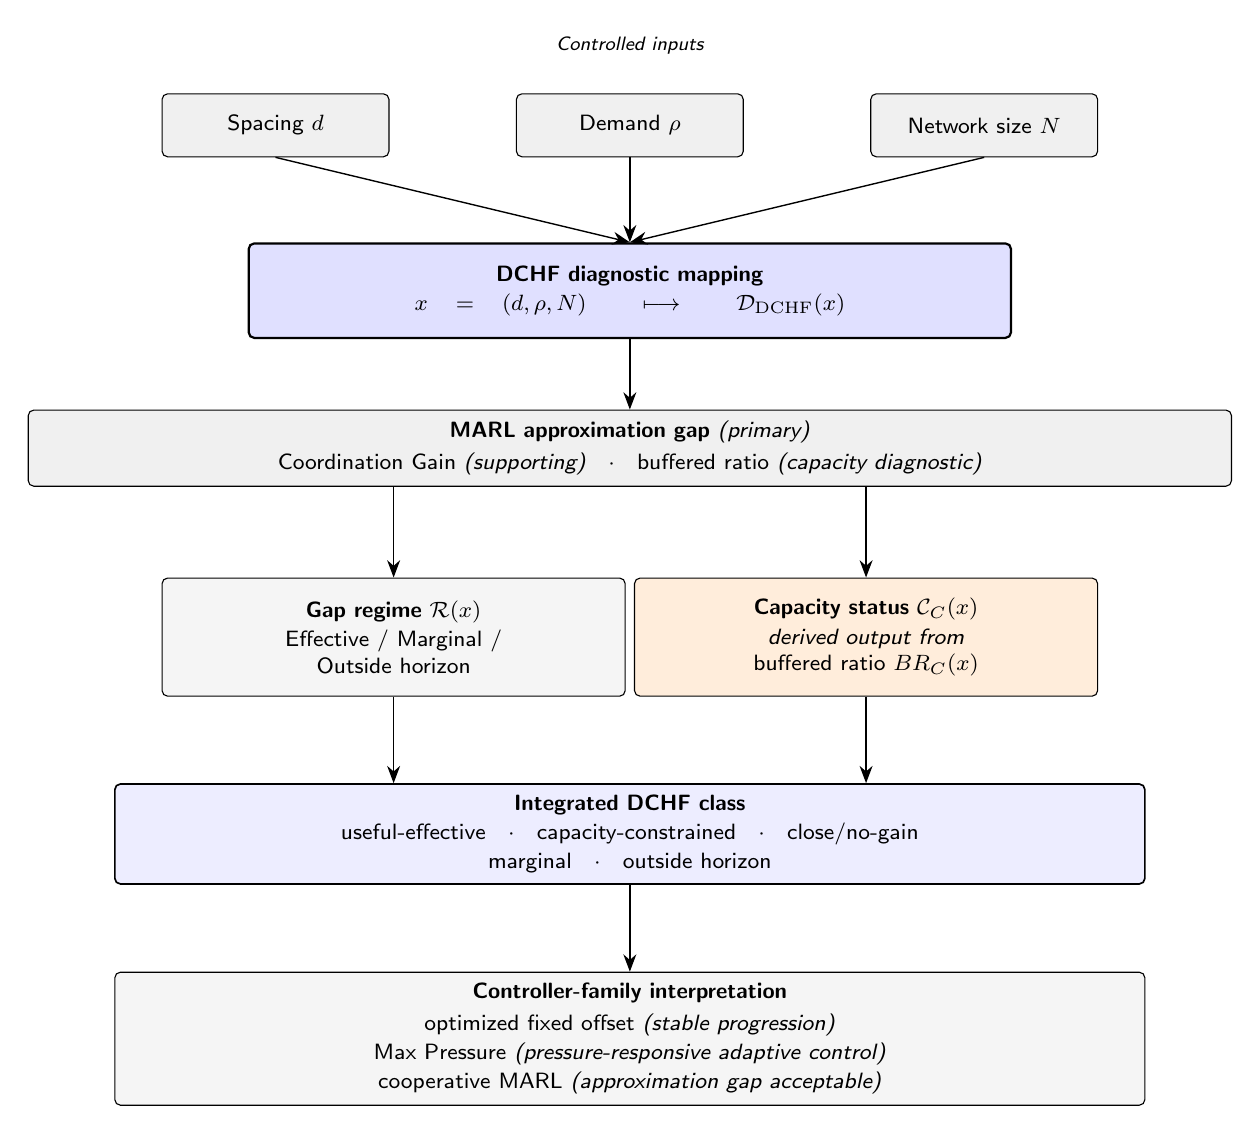
\begin{tikzpicture}[
  font=\footnotesize\sffamily,
  >={Stealth[length=2.2mm]},
  box/.style={draw=black, rounded corners=2pt, align=center, inner sep=4pt, line width=0.4pt},
  inp/.style={box, fill=black!6, minimum height=8mm, text width=26mm},
  core/.style={box, fill=blue!12, line width=0.8pt, text width=94mm, minimum height=12mm},
  diag/.style={box, fill=black!6, text width=150mm, minimum height=9mm},
  regime/.style={box, fill=black!4, text width=56mm, minimum height=15mm},
  capout/.style={box, fill=orange!14, text width=56mm, minimum height=15mm},
  klass/.style={box, fill=blue!7, line width=0.6pt, text width=128mm, minimum height=11mm},
  interp/.style={box, fill=black!4, text width=128mm, minimum height=13mm},
  ar/.style={->, line width=0.5pt},
]
\node[inp] (i1) at (0,0) {Spacing $d$};
\node[inp] (i2) at (4.5,0) {Demand $\rho$};
\node[inp] (i3) at (9,0) {Network size $N$};
\node[font=\scriptsize\sffamily\itshape, anchor=south] at (4.5,0.78) {Controlled inputs};
\node[core] (core) at (4.5,-2.1) {\textbf{DCHF diagnostic mapping}\\[1pt]$x=(d,\rho,N)\;\longmapsto\;\mathcal{D}_{\mathrm{DCHF}}(x)$};
\node[diag] (diag) at (4.5,-4.1) {\textbf{MARL approximation gap} \emph{(primary)}\\[2pt]Coordination Gain \emph{(supporting)} \; $\cdot$ \; buffered ratio \emph{(capacity diagnostic)}};
\node[regime] (reg) at (1.5,-6.5) {\textbf{Gap regime} $\mathcal{R}(x)$\\[1pt]Effective / Marginal /\\ Outside horizon};
\node[capout] (cap) at (7.5,-6.5) {\textbf{Capacity status} $\mathcal{C}_C(x)$\\[1pt]\emph{derived output from}\\ buffered ratio $BR_C(x)$};
\node[klass] (kl) at (4.5,-9.0) {\textbf{Integrated DCHF class}\\[1pt]useful-effective \; $\cdot$ \; capacity-constrained \; $\cdot$ \; close/no-gain\\[1pt]marginal \; $\cdot$ \; outside horizon};
\node[interp] (int) at (4.5,-11.6) {\textbf{Controller-family interpretation}\\[2pt]optimized fixed offset \emph{(stable progression)}\\[1pt]Max Pressure \emph{(pressure-responsive adaptive control)}\\[1pt]cooperative MARL \emph{(approximation gap acceptable)}};
\draw[ar] (i1.south) -- (core.north);
\draw[ar] (i2.south) -- (core.north);
\draw[ar] (i3.south) -- (core.north);
\draw[ar] (core.south) -- (diag.north);
\draw[ar] (diag.south) -- (diag.south -| reg.north) -- (reg.north);
\draw[ar] (diag.south) -- (diag.south -| cap.north) -- (cap.north);
\draw[ar] (reg.south) -- (kl.north -| reg.south);
\draw[ar] (cap.south) -- (kl.north -| cap.south);
\draw[ar] (kl.south) -- (int.north);
\end{tikzpicture}%
}
\caption{Conceptual architecture of the Dynamic Coordination Horizon Framework (framework illustration, not an experimental result). Controlled conditions $x=(d,\rho,N)$ are mapped to the integrated diagnosis $\mathcal{D}_{\mathrm{DCHF}}(x)$ through three diagnostics---the MARL approximation gap (primary), the Coordination Gain (supporting), and the buffered ratio (capacity). The gap regime $\mathcal{R}(x)$ and the derived capacity status $\mathcal{C}_C(x)$ recombine into the five integrated DCHF classes (useful-effective, capacity-constrained, close/no-gain, marginal, outside horizon). Capacity is a diagnostic output derived from the buffered ratio, not an independently controlled input.}
\label{fig:dchf_conceptual_framework}
\end{figure}

\FloatBarrier
\subsubsection{Operating conditions and Coordination Gain (supporting indicator)}
\label{subsubsec:cg_surface}

An experimental condition is $x=(d,\rho,N)$, where $d$ is spacing, $\rho$ is demand intensity, and $N$ is the number of controlled intersections. Coordination usefulness is represented by the mapping
\[
x\longmapsto\mathcal{D}_{\mathrm{DCHF}}(x),
\]
studied through one-dimensional projections. Capacity is not an independently controlled coordinate: for controller $C$, the observed capacity state $\mathcal{C}_C(x)$ is derived from its buffered ratio $BR_C(x)$. Coordination Gain is the supporting indicator: with $J_{\mathrm{sim}}(x)$ the mean total waiting time of simultaneous fixed-time control and $J_C(x)$ that of controller $C$, for lower-is-better metrics
\begin{equation}
CG_C(x)=\left(1-\frac{J_C(x)}{J_{\mathrm{sim}}(x)}\right)\times 100 .
\label{eq:coordination_gain}
\end{equation}
Mean total waiting time is the primary cost; speed, queue, vehicle count, and buffering are reported in support.

\subsubsection{Benchmark-relative coordination diagnosis: the MARL approximation gap}
\label{subsubsec:marl_gap}

The MARL approximation gap is the primary diagnostic. The two indicators answer different questions: Coordination Gain asks \textit{does coordination improve over simultaneous fixed-time control?}, the approximation gap asks \textit{how close does cooperative MARL come to the best tested benchmark?} A learned controller can satisfy the first while failing the second. The optimized fixed-offset benchmark $J_{\mathrm{off}}^{*}(x)=\min_{\Delta}J_{\mathrm{off}}(x,\Delta)$ is obtained by exhaustive sweep over $\Delta\in\{0,5,\ldots,90\}$~s (a $19\times19$ sweep over $J_2,J_3$ for three-intersection corridors). At $N=5$ the benchmark is instead a one-parameter cumulative progression-offset benchmark, swept over a base increment $b$ on the same $5$~s grid and applied as $\Delta_i=((i-1)b)\bmod90$ at intersection $i$ (Section~\ref{subsec:n5_scalability}); the $N=5$ comparator is therefore the best plan within that restricted family rather than a fully optimized offset vector. With this qualification,
\begin{equation}
G_{\mathrm{QMIX}}(x)=
\frac{J_{\mathrm{QMIX}}(x)-J_{\mathrm{off}}^{*}(x)}{J_{\mathrm{off}}^{*}(x)}
\times 100 .
\label{eq:qmix_gap}
\end{equation}
In multi-seed experiments the gap is a seed-averaged quantity and its interval is a paired bootstrap over seed indices. Because paired per-seed averaging and direct evaluation of Eq.~\eqref{eq:qmix_gap} at the reported seed-averaged waiting measures agree to within $0.07$ percentage points throughout the paired five- and ten-seed comparisons reported here, and to within $0.3$ percentage points in the exploratory three-seed cycle probe of Supplementary Section~S-3, no tabulated regime classification depends on the choice. A positive gap means QMIX is worse than the benchmark, a negative gap slightly better. Where Max Pressure is evaluated, an analogous gap places it in the same framework:
\begin{equation}
G_{\mathrm{MP}}(x)=
\frac{J_{\mathrm{MP}}(x)-J_{\mathrm{off}}^{*}(x)}{J_{\mathrm{off}}^{*}(x)}
\times 100 .
\label{eq:max_pressure_gap}
\end{equation}
A negative $G_{\mathrm{MP}}$ means that Max Pressure produces a
lower waiting measure than the best tested fixed-offset plan, whereas
a positive value indicates that the optimized fixed-offset benchmark
performs better. Reporting $G_{\mathrm{MP}}$ alongside
$G_{\mathrm{QMIX}}$ permits a common comparison of the learned,
pressure-responsive, and fixed-offset controllers and indicates how
competitive the fixed-offset benchmark remains under each operating condition.

\subsubsection{Regime and capacity classification}
\label{subsubsec:coordination_regime}

Coordination regimes are classified directly from the approximation gap:
\begin{equation}
\mathcal{R}(x)=
\begin{cases}
\text{Effective},  & G_{\mathrm{QMIX}}(x)\leq 5\%,\\
\text{Marginal},   & 5\% < G_{\mathrm{QMIX}}(x)\leq 10\%,\\
\text{Outside horizon}, & G_{\mathrm{QMIX}}(x)>10\% .
\end{cases}
\label{eq:coordination_regime}
\end{equation}
The rule is $G_{\mathrm{QMIX}}\leq\delta$ (not $|G|\leq\delta$), so a negative gap is always effective. For any controller $C$, the same thresholds define a controller-relative regime $\mathcal{R}_C(x)$; $\mathcal{R}(x)\equiv\mathcal{R}_{\mathrm{QMIX}}(x)$ unless a controller is named explicitly, and Max~Pressure regimes are written $\mathcal{R}_{\mathrm{MP}}$. The $5\%$ reference level is grounded in the benchmark's own offset insensitivity rather than chosen arbitrarily: at the turning-movement horizon anchor
($d=300$~m, medium demand) the waiting-time-optimal offset is $45$~s, and offsets within roughly $\pm5$~s of it ($40$--$50$~s) all remain within $5\%$ of the optimum, whereas offsets outside this band degrade sharply (Figure~\ref{fig:offset_sweep_threshold_curve}). A controller within $5\%$ of the optimum is therefore operating inside the range of offsets the benchmark itself treats as near-equivalent, consistent with the flat minimum of classical delay models~\cite{webster1958,sadegh1988comparative}; the $10\%$ outer bound provides a deliberately wider tolerance marking a clear departure from the optimized benchmark. Both are pre-specified interpretation tolerances, neither universal nor data-independent. Under the explicit $\delta\in\{3\%,5\%,10\%\}$ sensitivity analysis, the exact membership of the effective set shifts under the strict $3\%$ tolerance---only the tested $300$~m point remains spatially effective---whereas the demand membership is unchanged between $3\%$ and $5\%$ and the third-light classifications are the most threshold-sensitive. The broader conclusions of sparse fixed-policy effectiveness concentrated at intermediate spacing, and of conditional scalability, are unchanged across the tested range. A full derivation of the threshold anchors is given in Supplementary Section~S-1.

\begin{figure}[!htbp]
\centering

\includegraphics[width=0.55\textwidth]{figures/offset_sweep_threshold_curve.pdf}
\caption{Offset-sweep response at the turning-movement horizon anchor
($d=300$~m, medium demand): mean total waiting time versus offset. The optimum is at $45$~s; the shaded band marks offsets within $5\%$ of the optimum ($40$--$50$~s). The $5\%$ effectiveness threshold coincides with this empirical flat-minimum bandwidth.}
\label{fig:offset_sweep_threshold_curve}
\end{figure}

Physical capacity can limit performance independently of coordination quality, so a small gap under congestion need not indicate good coordination. For controller $C$, the buffered ratio
\[
BR_C(x)=
\frac{N_{\mathrm{buffered},C}(x)}
     {N_{\mathrm{expected}}(x)}
\]
diagnoses the observed capacity state:
\begin{equation}
\mathcal{C}_C(x)=
\begin{cases}
\text{Unconstrained},           & BR_C(x)<0.01,\\
\text{Mild insertion pressure}, & 0.01\leq BR_C(x)<0.10,\\
\text{Capacity-limited},        & 0.10\leq BR_C(x)<0.25,\\
\text{Oversaturated},           & BR_C(x)\geq0.25.
\end{cases}
\label{eq:capacity_regime}
\end{equation}
Unless another controller is named explicitly, $BR(x)\equiv BR_{\mathrm{QMIX}}(x)$ and $\mathcal{C}(x)\equiv\mathcal{C}_{\mathrm{QMIX}}(x)$.
\begin{equation}
H_B^{C}=\left\{\,x \mid BR_C(x)<0.25\,\right\},
\qquad H_B\equiv H_B^{\mathrm{QMIX}}.
\label{eq:buffered_ratio}
\end{equation}
Here $N_{\mathrm{buffered},C}$ is the number of route-file vehicles that have not been inserted into the network by the end of the $3600$~s horizon (the SUMO insertion backlog at simulation end) under controller $C$, and $N_{\mathrm{expected}}$ is the total route-file demand. The buffered ratio operationalizes a queue-storage criterion grounded in the Cell Transmission Model~\cite{daganzo1994cell}: once storage between two intersections is exceeded, spillback couples them regardless of coordination quality. The $BR_C=0.25$ threshold defines the boundary of the controller-specific capacity-feasible set and serves as a deliberately conservative operational cut-off for oversaturation; the intermediate interval $0.10 \le BR_C(x) < 0.25$ is classified as capacity-limited but remains within $H_B^C$, because increasing storage constraints influence coordination performance without yet indicating complete capacity breakdown. Boundary cases either lie well below this threshold or are reported together with their buffered ratio, so the qualitative conclusions do not depend on its exact numerical value. For the observed joint grid, the three approximation-effective cells classified as useful-effective have $BR_{\mathrm{QMIX}}\leq0.065$, whereas the three approximation-effective cells classified as capacity-constrained have $BR_{\mathrm{QMIX}}\geq0.20$. Consequently, the reported integrated class counts are invariant to any capacity-precedence threshold chosen between these two observed groups. This empirical separation supports the robustness of the reported map, although it does not establish $0.10$ as a universal capacity-pressure boundary.

The buffered ratio measures demand that cannot enter the network; it does not by
itself separate queue accumulation from physical link blockage. A complementary
spillback indicator is therefore logged: the \emph{central-link occupancy} is the
number of vehicles present on the link between the two signals divided by its
storage capacity, computed per direction as the link length divided by a
$7.5$~m vehicle storage space ($5$~m vehicle plus $2.5$~m minimum gap) and taken
as the larger of the two directional ratios. An occupancy of at least $80\%$ is
recorded as a spillback event. This threshold is never exceeded by any tested controller at any tested demand level---the highest observed central-link occupancy is $0.470$, well below the criterion (Supplementary Section~S-10)---so the high-demand failure mode diagnosed here is queue accumulation under capacity pressure rather than blockage of the central link.

Reporting $\mathcal{R}(x)$ and $\mathcal{C}(x)$ together prevents a capacity-bound condition from being misread as algorithmic failure. Because $BR_C$ is measured for the controller under evaluation, a capacity-limited or oversaturated classification indicates limited residual insertion margin for that controller under its own cycle, phase, and service constraints within the finite evaluation horizon; it does not imply that the physical network is saturated for every controller family. The optimized offset and QMIX share the same fixed cycle, whereas Max Pressure belongs to a pressure-responsive family, so reporting $G_{\mathrm{MP}}$ alongside $G_{\mathrm{QMIX}}$ places both on a common fixed-offset reference scale and separates controller-family limitations from network-capacity limitations.
\subsubsection{Horizon definitions and integrated diagnosis}
\label{subsubsec:horizon_definitions}

With $H_B$ already defined by the buffered-ratio cutoff in
Eq.~\eqref{eq:buffered_ratio}, the remaining gap-based horizons are defined as
one-dimensional projections of the operating condition
$x=(d,\rho,N)$. Let $x_S(d)$, $x_D(\rho)$, and $x_N(N)$ denote the spatial,
demand, and scalability experimental slices, respectively, with non-varied
components fixed to their stated reference values; for $x_N(N)$ the policy is
trained at the tested network size. Then
\begin{equation}
\begin{aligned}
H_S(\delta)&=\{\,d:G_{\mathrm{QMIX}}(x_S(d))\leq\delta\,\},\\
H_D(\delta)&=\{\,\rho:G_{\mathrm{QMIX}}(x_D(\rho))\leq\delta\,\},\\
H_N(\delta)&=\{\,N:G_{\mathrm{QMIX}}(x_N(N))\leq\delta\,\}.
\end{aligned}
\label{eq:horizon_defs}
\end{equation}
Practical usefulness is determined by the integrated DCHF classification, which additionally considers Coordination Gain and controller-specific capacity status.

Because only $N\in\{2,3,5\}$ are tested, the upper scalability boundary is not located; whether each tested network size lies inside $H_N(5\%)$ is established empirically in Sections~\ref{subsec:multiseed_scenario_a}, \ref{subsec:scalability}, and \ref{subsec:n5_scalability}. The three diagnostics combine into a single integrated DCHF signature:
\begin{equation}
\boxed{\;\mathcal{D}_{\mathrm{DCHF}}(x)=
\bigl(G_{\mathrm{QMIX}}(x),\;CG_{\mathrm{QMIX}}(x),\;
\mathcal{C}_{\mathrm{QMIX}}(x)\bigr)\;}
\label{eq:integrated_dchf_diagnosis}
\end{equation}
which separates five operational cases: (i) useful effective, when $G_{\mathrm{QMIX}}\leq5\%$, $CG_{\mathrm{QMIX}}>0$, and $BR_{\mathrm{QMIX}}<0.10$; (ii) capacity-constrained effective, when $G_{\mathrm{QMIX}}\leq5\%$ and $BR_{\mathrm{QMIX}}\geq0.10$; (iii) close/no-gain, when $G_{\mathrm{QMIX}}\leq5\%$, $CG_{\mathrm{QMIX}}\leq0$, and $BR_{\mathrm{QMIX}}<0.10$; (iv) marginal, when $5\%<G_{\mathrm{QMIX}}\leq10\%$; and (v) outside the horizon, when $G_{\mathrm{QMIX}}>10\%$. Mild insertion pressure therefore remains eligible for either the useful-effective or close/no-gain class. The useful-effective class denotes benchmark closeness, positive performance relative to simultaneous fixed-time control, and absence of material insertion pressure under the stated rule. It does not by itself establish causal benefit from inter-agent cooperation or superiority over every evaluated controller family. The corresponding optimized-offset opportunity score is therefore reported separately. Conditions in which the optimized offset yields little or no improvement over simultaneous fixed-time control are interpreted as lacking a material fixed-offset coordination opportunity, irrespective of the gap value. Capacity precedence applies only within the approximation-effective branch; marginal and outside-horizon conditions retain their gap-based labels, with capacity status reported alongside them. The buffered ratio underlying every capacity diagnosis is reported in the capacity-diagnosis tables and component heatmaps of Supplementary Section~S-10.
\subsubsection{Coordination-opportunity score and fixed-policy generalization horizon}
\label{subsubsec:gen_horizon}

Two related but distinct questions are considered. First, the
\emph{coordination-opportunity score} is Eq.~\eqref{eq:coordination_gain}
evaluated for the optimized offset,
$CG_{\mathrm{off}}(x)=\bigl(1-J_{\mathrm{off}}^{*}(x)/J_{\mathrm{sim}}(x)\bigr)\times100$,
quantifying the progression benefit available under the best tested
fixed-offset plan relative to simultaneous fixed-time operation. It is
independent of the evaluated learned policy but remains benchmark-dependent,
since the opportunity is quantified using the best tested fixed-offset plan
under a fixed cycle and green split rather than an absolute traffic-control
optimum, and is retained as a continuous magnitude rather than a binary
horizon. Second, the \emph{fixed-policy generalization horizon} is defined for
a reference policy $\pi_{\mathrm{ref}}$, trained once at reference condition
$x_0$ and evaluated elsewhere without retraining:
\begin{equation}
G^{\mathrm{gen}}_{\pi_{\mathrm{ref}}}(x)=
\frac{J_{\pi_{\mathrm{ref}}}(x)-J_{\mathrm{off}}^{*}(x)}{J_{\mathrm{off}}^{*}(x)}
\times 100,\qquad
H_{\mathrm{gen}}(\pi_{\mathrm{ref}})=\{x : G^{\mathrm{gen}}_{\pi_{\mathrm{ref}}}(x)\leq\delta\},
\label{eq:gen_horizon}
\end{equation}
subject to the capacity-precedence qualification, with the learned policy held
fixed while the fixed-offset benchmark is re-optimized per condition. The spatial and demand sweeps are accordingly designed to estimate this
generalization envelope rather than a frontier obtained by retraining per
condition; whether condition-specific retraining would alter the effective
region is outside the scope of the present study.
\subsubsection{Theoretical grounding of the expected horizons}
\label{subsubsec:classical_prediction}

Classical coordination theory predicts that cooperation is not uniformly useful: short spacing yields storage interference; long spacing yields platoon dispersion and stale upstream information; low demand yields weak interaction; high demand yields capacity pressure. These expectations imply non-monotonic spatial and demand horizons and a conditional scalability horizon, which the results test against the optimized-offset benchmark. The supporting analytical constructs---a progression-offset estimate, a platoon-dispersion proxy, and an information-freshness function---are used as interpretive mechanisms rather than calibrated laws; Supplementary Section~S-6 provides a qualitative consistency check of the cohesion proxy against the observed spatial gap pattern, and Supplementary Section~S-7 gives the full notation.

In this use, spacing is not treated as the causal variable itself, but as an experimentally controlled proxy for latent traffic mechanisms---platoon cohesion, spillback risk, queue interaction, information freshness, and capacity pressure---that jointly determine whether coordination can be exploited. Consequently, the reported DCHF regions should be interpreted as operating regimes of the tested corridor family rather than universal geometric thresholds.

\subsection{Simulation Environment}
\label{subsec:simulation_env}

Experiments use synthetic aligned two-way arterial corridors, two lanes per approach with bidirectional main links. Synthetic geometry is intentional: it allows direct control of spacing, demand, corridor size, and turning composition, so controller differences can be interpreted relative to explicitly defined experimental factors rather than uncontrolled geometric complexity. Each signal runs a 90~s cycle (two 42~s green, two 3~s yellow), held fixed within the main experiments. In the spatial sweep, demand and movement composition are fixed while spacing varies; in the demand sweep, spacing and movement composition are fixed while demand varies. The same cycle applies to the simultaneous fixed-time, optimized-offset, and QMIX controllers, so the gap $G_{\mathrm{QMIX}}$ is not confounded by timing differences; absolute boundaries can shift under a substantially different cycle (Supplementary Section~S-3). Each run is 3600~s, with demand set by multipliers on a reference flow (low $0.5\times$ to oversaturation $2.5\times$).

Scenario~A is the through-movement corridor used to train and select QMIX~V2 and to conduct the reference controller comparisons. Scenario~B is the 70\%--15\%--15\% through/right/left transfer case on the original two-intersection geometry. The spatial, demand, and joint distance--demand horizon campaigns use generated corridor variants with the same movement split as Scenario~B.

\begin{figure}[!htbp]
\centering
\resizebox{\textwidth}{!}{%
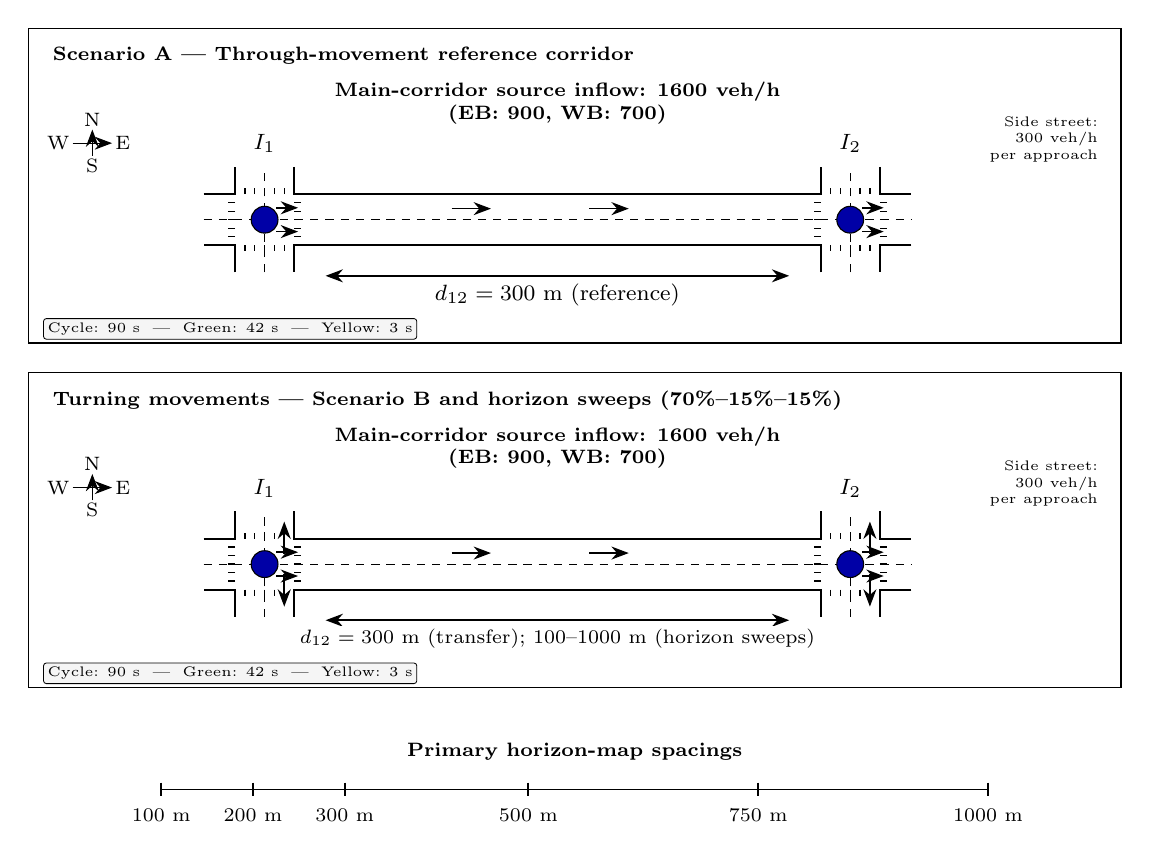
\begin{tikzpicture}[
    x=1.25cm,
    y=1.08cm,
    >={Stealth[length=2.2mm]},
    inkline/.style={line width=0.5pt, black},
    roadline/.style={line width=0.7pt, black},
    lanedash/.style={dashed, dash pattern=on 3pt off 2.5pt, line width=0.4pt, black},
    flow/.style={->, line width=0.6pt, black},
    turn/.style={->, line width=0.6pt, black},
    sig/.style={circle, fill=blue!65!black, draw=black, line width=0.4pt,
                minimum size=3.4mm, inner sep=0pt},
    dimarrow/.style={<->, line width=0.6pt, black},
    label/.style={font=\footnotesize},
    small/.style={font=\scriptsize},
    title/.style={font=\bfseries\scriptsize},
    sidebox/.style={font=\tiny, align=right, fill=white, inner sep=1pt},
    parambox/.style={draw=black, line width=0.3pt, fill=black!4,
                     rounded corners=1pt, inner sep=1.5pt, font=\tiny},
]
\newcommand{\intersection}[4]{%
  \begin{scope}[shift={(#1,#2)}]
    \def\rh{0.30}
    \def\arm{0.62}
    \fill[white] (-\arm,-\rh) rectangle (\arm,\rh);
    \fill[white] (-\rh,-\arm) rectangle (\rh,\arm);
    \draw[roadline] (-\arm,\rh) -- (-\rh,\rh) -- (-\rh,\arm);
    \draw[roadline] (\rh,\arm) -- (\rh,\rh) -- (\arm,\rh);
    \draw[roadline] (\arm,-\rh) -- (\rh,-\rh) -- (\rh,-\arm);
    \draw[roadline] (-\rh,-\arm) -- (-\rh,-\rh) -- (-\arm,-\rh);
    \draw[lanedash] (-\arm,0) -- (\arm,0);
    \draw[lanedash] (0,-\arm) -- (0,\arm);
    \foreach \i in {-2,-1,0,1,2}{
      \draw[inkline] (\i*0.10,\rh) -- (\i*0.10,\rh+0.07);
      \draw[inkline] (\i*0.10,-\rh) -- (\i*0.10,-\rh-0.07);
      \draw[inkline] (\rh,\i*0.10) -- (\rh+0.07,\i*0.10);
      \draw[inkline] (-\rh,\i*0.10) -- (-\rh-0.07,\i*0.10);
    }
    \node[sig] at (0,0) {};
    \node[label, anchor=south] at (0,\arm+0.05) {$#3$};
    \draw[flow] (0.12,0.14) -- (0.34,0.14);
    \draw[flow] (0.12,-0.14) -- (0.34,-0.14);
    \ifnum#4=1
      \draw[turn] (0.20,0.12) -- (0.20,0.50);
      \draw[turn] (0.20,-0.12) -- (0.20,-0.50);
    \fi
  \end{scope}
}
\newcommand{\panel}[3]{%
  \begin{scope}[shift={(0,#1)}]
    \def\panelw{11.1}
    \def\xL{2.4}
    \def\xR{8.35}
    \def\cy{1.45}
    \draw[inkline] (0,0) rectangle (\panelw,3.7);
    \node[title, anchor=north west] at (0.15,3.60) {#2};
    \node[small, anchor=north, align=center, font=\scriptsize\bfseries]
      at ({(\xL+\xR)/2},3.18)
      {Main-corridor source inflow: 1600 veh/h\\(EB: 900, WB: 700)};
    \intersection{\xL}{\cy}{I_1}{#3}
    \intersection{\xR}{\cy}{I_2}{#3}
    \draw[roadline] (\xL+0.62,\cy+0.30) -- (\xR-0.62,\cy+0.30);
    \draw[roadline] (\xL+0.62,\cy-0.30) -- (\xR-0.62,\cy-0.30);
    \draw[lanedash] (\xL+0.62,\cy) -- (\xR-0.62,\cy);
    \draw[flow] (\xL+1.9,\cy+0.13) -- (\xL+2.3,\cy+0.13);
    \draw[flow] (\xL+3.3,\cy+0.13) -- (\xL+3.7,\cy+0.13);
    \draw[dimarrow] (\xL+0.62,\cy-0.66) -- (\xR-0.62,\cy-0.66);
    \ifnum#3=0
      \node[label, anchor=north, fill=white, inner sep=1pt]
        at ({(\xL+\xR)/2},\cy-0.72)
        {$d_{12}=300$~m (reference)};
    \else
      \node[small, anchor=north, fill=white, inner sep=1pt]
        at ({(\xL+\xR)/2},\cy-0.72)
        {$d_{12}=300$~m (transfer); 100--1000~m (horizon sweeps)};
    \fi
    \node[sidebox, anchor=north east]
      at ({\panelw-0.20},2.70) {Side street:\\300 veh/h\\per approach};
    \begin{scope}[shift={(0.65,2.25)}]
      \draw[->,line width=0.4pt] (0,-0.05) -- (0,0.26) node[small,above,inner sep=1pt]{N};
      \draw[->,line width=0.4pt] (-0.20,0.10) -- (0.20,0.10);
      \node[small,left,inner sep=1pt] at (-0.20,0.10){W};
      \node[small,right,inner sep=1pt] at (0.20,0.10){E};
      \node[small,below,inner sep=1pt] at (0,-0.05){S};
    \end{scope}
    \node[parambox, anchor=south west] at (0.15,0.04)
      {Cycle: 90~s \;|\; Green: 42~s \;|\; Yellow: 3~s};
  \end{scope}
}
\panel{4.15}{Scenario A --- Through-movement reference corridor}{0}
\panel{0.10}{Turning movements --- Scenario B and horizon sweeps (70\%--15\%--15\%)}{1}
\begin{scope}[shift={(0,-0.95)}]
  \node[title] at (5.55,0.30) {Primary horizon-map spacings};
  \def\xa{1.35}\def\xb{9.75}
  \draw[line width=0.7pt] (\xa,-0.15) -- (\xb,-0.15);
  \foreach \s/\f in {100/0,200/0.111,300/0.222,500/0.444,750/0.722,1000/1.0}{
    \draw[line width=0.7pt]
      ({\xa+\f*(\xb-\xa)},-0.07) -- ({\xa+\f*(\xb-\xa)},-0.23);
    \node[small, anchor=north] at ({\xa+\f*(\xb-\xa)},-0.26) {\s~m};
  }
\end{scope}
\end{tikzpicture}%
}
\caption{Experimental two-intersection configurations. Scenario~A
(top) is the through-movement training and reference-comparison corridor
at $d_{12}=300$~m. The turning-movement configuration (bottom), with a
70\%--15\%--15\% through/right/left split, is used for the Scenario~B
transfer at $d_{12}=300$~m and for the generated spatial, demand, and
joint distance--demand horizon variants. The six primary horizon-map spacings are 100, 200, 300, 500,
750, and 1000~m; the paired spatial validation adds a 450~m
boundary-infill point
(Table~\ref{tab:experimental_factors}). The $N=3$ and $N=5$
extensions append downstream signals at the stated homogeneous spacing under through movements.}
\label{fig:corridor_geometry}
\end{figure}

The full list of experimental factors and tested levels is given in Table~\ref{tab:experimental_factors}.

\FloatBarrier
\subsection{Compared Control Strategies}
\label{subsec:control_strategies}
The two-intersection evidence is organized in two stages. First, a seven-strategy single-seed Scenario~A screening compares simultaneous fixed-time control, the optimized fixed offset, queue-based adaptive control, Independent DQN, and QMIX variants V1--V3, with simultaneous fixed-time (zero relative offset) serving as the uncoordinated reference for Coordination Gain. Second, the optimized offset, the selected QMIX~V2 policy, and Max Pressure are evaluated in the formal ten-seed reference comparison. Table~\ref{tab:control_strategies_summary} additionally lists the controlled VDN mixer ablation and the three- and five-agent QMIX extensions used in the scalability experiments. The optimized fixed-offset benchmark and Max Pressure require additional methodological specification, while the learning-based controllers are briefly introduced below. \textbf{Optimized fixed-offset} applies the best swept offset $\Delta\in\{0,5,\ldots,90\}$~s and is the benchmark for the approximation gap. \textbf{Max Pressure}~\cite{varaiya2013max,ducrocq2023deep} is an acyclic, non-learning adaptive controller that, after each minimum-green interval, activates the phase of maximum pressure:
\begin{equation}
P_i(p,t)=\sum_{(l,m)\in\mathcal{M}_i(p)}\bigl[n_l(t)-n_m(t)\bigr],
\label{eq:max_pressure}
\end{equation}
where $\mathcal{M}_i(p)$ is the set of incoming--outgoing lane pairs served by phase $p$ at intersection $i$, and $n_l(t),n_m(t)$ are the incoming and outgoing lane counts. In Scenario~A it uses $T_{g,\min}=10$~s and yellow $T_y=3$~s and requires real-time detection on both incoming and outgoing lanes, providing a strong pressure-based adaptive reference distinct from progression-based coordination. These operational constraints---minimum green, fixed yellow, and two aggregated phases over a finite $3600$~s horizon---distinguish the implemented controller from the idealized formulation used in the canonical stability analysis, so it is treated here as a strong empirical baseline rather than as an instance inheriting the formal maximum-stability guarantee. Among the learning-based controllers (Table~\ref{tab:control_strategies_summary}), \textbf{single-agent DQN}~\cite{Mnih2015} validates the SUMO--TraCI--RL loop at $N=1$ and \textbf{Independent DQN} assigns one local agent per intersection with no shared value function. \textbf{QMIX}~\cite{Rashid2018} is evaluated in three variants (V1--V3) in Scenario~A, with QMIX~V2 selected on the primary waiting-time criterion (Section~\ref{subsec:scenario_a}) and retained for all two-intersection DCHF experiments; the three- and five-agent scalability policies use the same observation and network template but are trained from scratch at their own network sizes.
 This benchmark set is a deliberate choice of \emph{transparent, exactly reproducible} references rather than the strongest conceivable classical controllers: the optimized fixed offset and Max Pressure are both reconstructable from the reported settings, whereas a deployed adaptive system (SCOOT, SCATS) or a state-of-the-art learned controller (e.g.\ MPLight, CoLight) carries implementation-specific tuning that would confound the benchmark-relative gap; extending the diagnostic to those controllers is identified as future work (Section~\ref{sec:future_roadmap}).

\begin{table}[H]
\centering
\caption{Compared control strategies and their methodological roles.}
\label{tab:control_strategies_summary}
\resizebox{\textwidth}{!}{%
\begin{tabular}{p{3.5cm}p{5.0cm}p{5.3cm}}
\toprule
\textbf{Strategy} & \textbf{Information used} & \textbf{Methodological role} \\
\midrule
Simultaneous fixed-time & No coordination information & Uncoordinated reference for Coordination Gain. \\
Optimized fixed offset & Offline offset sweep & Classical benchmark for the approximation gap. \\
Queue-based adaptive & Local instantaneous queues & Local adaptivity without temporal coordination. \\
Max Pressure & Real-time incoming/outgoing lane counts & Strong non-learning pressure-based baseline. \\
Single-agent DQN & Local state only & Validates the SUMO--TraCI--RL pipeline at $N=1$. \\
Independent DQN & Local observations, independent learning & Learning without cooperative decomposition. \\
QMIX V1--V3 & Local observations + global state (training) & Configuration selection at $N=2$; V2 retained as the reference variant. \\
VDN & Local observations + global state (training) & Additive-mixer ablation of QMIX (Section~\ref{subsubsec:vdn_ablation}). \\
Three-/five-agent QMIX & Centralized training, decentralized execution & Bounded scalability tests at $N=3,5$. \\
\bottomrule
\end{tabular}%
}
\end{table}

\subsection{Training and Evaluation Protocol}
\label{subsec:training_evaluation_protocol}

Before the corridor experiments, the SUMO--TraCI--RL pipeline was validated at an isolated signalized intersection; DQN~V2 was competitive with safe fixed-time control on the network-level waiting measure, and the full DQN~V1/V2 comparison is reported in Supplementary Section~S-3. Independent DQN learns one local value function per intersection; QMIX trains all agents through a mixing network that combines local action-values into a joint value $Q_{\mathrm{tot}}(s,\mathbf{a})$ from the global state during training, while execution uses only local observations (full formulation in Supplementary Section~S-8). The selected reference variant is reused across the horizon experiments without per-condition retuning. Evaluation runs with exploration disabled.

Unless explicitly stated otherwise, the reported multi-seed statistics for learned controllers use common SUMO evaluation seeds for fixed trained policies. They therefore quantify robustness to traffic-realization stochasticity under a trained policy, not full training-run variability over independent neural-network initializations, replay histories, and exploration trajectories. Single-seed runs support exploratory horizon mapping; ten paired evaluation seeds support the Scenario~A reference and Scenario~B transfer comparisons; five paired evaluation seeds support the boundary-defining spatial and demand cases, the Max Pressure sweeps, and the five-intersection validation. Computational costs (all experiments run on CPU) are reported in Supplementary Section~S-2.

\subsection{Experimental Design}
\label{sec:experimental_design}

\subsubsection{Experimental Factors}

Table~\ref{tab:experimental_factors} lists the factors and tested levels. The medium reference demand totals 2{,}800~veh/h: 900~veh/h eastbound and 700~veh/h westbound on the main corridor, plus 300~veh/h from each of four side approaches; in the turning-movement variants the main-corridor straight-through components are 630 and 490~veh/h. With a 90~s cycle, 42~s of main-corridor effective green ($g/C\approx0.47$), and a nominal saturation flow of 1{,}800~veh/h/lane, the two-lane effective-green capacity of the critical eastbound approach is $2\times1{,}800\times(42/90)=1{,}680$~veh/h, which yields the $v/c$ values listed in the table.

\begin{table}[!htbp]
\centering
\caption{Experimental factors and tested levels.}
\label{tab:experimental_factors}
\small
\setlength{\tabcolsep}{5pt}
\begin{tabularx}{\textwidth}{p{3.4cm}Y}
\toprule
\textbf{Factor} & \textbf{Tested levels} \\
\midrule
Two-intersection distance $d_{12}$ &
100, 200, 300, 500, 750, 1000~m. These six spacings define the single-seed
exploratory map and the joint distance--demand grid ($6\times5=30$ cells).
The paired five-seed spatial validation sweep additionally includes a
450~m boundary-infill point, evaluated to resolve the effective-to-marginal
transition of $H_S$ between 300 and 500~m; it is not part of the 30-cell grid. \\
Demand level $\rho$ &
Low ($0.5\times$), medium ($1.0\times$), high ($1.5\times$),
saturation ($2.0\times$), oversaturation ($2.5\times$), applied as multipliers
on the medium reference flow of 2{,}800~veh/h. The corresponding approximate
$v/c$ values are $0.27$, $0.54$, $0.80$, $1.07$, and $1.34$. \\
Number of intersections $N$ &
$N=1$ pipeline validation; $N=2$ reference; $N=3,5$ scalability. \\
Third-light distance $d_{23}$ &
100--1000~m with $d_{12}=300$~m fixed. \\
Turning configuration &
Scenario~A reference and training: through movements. Scenario~B transfer and
the generated spatial, demand, and joint distance--demand horizon variants:
turning movements at $d_{12}=300$~m (Figure~\ref{fig:corridor_geometry}).
The $N=3$ and $N=5$ scalability corridors use through movements. \\
Control strategy &
\textit{Classical:} fixed-time, optimized offset, queue-adaptive, Max Pressure.
\textit{Learning:} single-agent DQN, Independent DQN, QMIX V1--V3, VDN, and
three- and five-agent QMIX. \\
Random seeds &
Single-seed exploratory mapping; ten-seed validation in Scenario~A and Scenario~B;
five-seed paired validation for boundary and Max Pressure sweeps. \\
\bottomrule
\end{tabularx}
\end{table}

\subsubsection{Experimental Phases}

The study progresses from single-intersection pipeline validation (Supplementary Section~S-3) through the two-intersection reference, transfer, spatial, demand, and joint distance--demand experiments to the $N=3$ and $N=5$ scalability tests and the paired Max Pressure sweeps, all reported in Section~\ref{sec:results_discussion}. Because the campaigns combine different levels of statistical strength, Table~\ref{tab:evidence_levels} makes the evidence basis of each result explicit.

\begin{table}[!htbp]
\centering
\caption{Evidence levels and validation scope across the experimental campaign.}
\label{tab:evidence_levels}
\small
\setlength{\tabcolsep}{4pt}
\renewcommand{\arraystretch}{1.08}

\begin{tabularx}{\textwidth}{
@{}
>{\raggedright\arraybackslash}p{0.29\textwidth}
>{\raggedright\arraybackslash}p{0.16\textwidth}
>{\raggedright\arraybackslash}X
@{}
}
\toprule
\textbf{Experiment} &
\textbf{Seeds} &
\textbf{Statistical scope} \\
\midrule

Scenario A: optimized offset, QMIX V2, and Max Pressure &
10 paired &
Paired Wilcoxon tests and bootstrap confidence intervals;
strongest comparative evidence. \\

Scenario B transfer &
10 paired &
Paired Wilcoxon tests and bootstrap confidence intervals. \\

Scenario B budget and initialization ablations &
5 evaluation seeds per fixed policy &
Mean, standard deviation, and bootstrap confidence interval.
Each ablation uses one trained checkpoint, so variability concerns
traffic realizations rather than independent training runs. \\

Max Pressure spatial and demand sweeps &
5 paired &
All three controllers evaluated with common seeds;
bootstrap confidence intervals for the benchmark-relative gaps. \\

Spatial and demand boundary conditions &
5 paired &
Bootstrap confidence intervals for the approximation gap and
regime-stability assessment. \\

$N=5$ reference validation &
5 paired &
Mean and standard deviation for the bounded scalability comparison
against the cumulative progression-offset benchmark. \\

Max Pressure at $N=3$ and $N=5$ &
5 evaluation seeds &
Max Pressure mean and standard deviation compared with the available
offset and QMIX reference results; diagnostic evidence. \\

Joint grid: validated cells &
5 paired &
Fifteen of 30 cells, including the boundary and useful-effective
conditions; bootstrap confidence intervals for the approximation gap. \\

Joint grid: remaining cells &
1 &
Fifteen of 30 cells retained as exploratory point estimates. \\

$N=3$ reference, third-light sweep, and $N=5$ stress grid &
1, except where stated &
Single-seed exploratory mapping; the $N=3$ reference condition is
additionally evaluated over five seeds in the supplementary analysis. \\

\bottomrule
\end{tabularx}
\end{table}

\subsection{Performance Metrics}
\label{sec:metrics}

Conventional traffic metrics (Supplementary Section~S-11) quantify operational performance; the DCHF indicators, defined in Section~\ref{subsec:dchf}, classify each condition as effective, marginal, capacity-constrained, or outside the useful horizon.

Mean total waiting time is the primary indicator because it reflects delay accumulation and is sensitive to both local queueing and corridor-level coordination. Operationally, for controller $C$ under condition $x$,
\begin{equation}
J_C(x) = \frac{1}{T}\sum_{s=1}^{T}\sum_{v \in V_s} w_v(s),
\label{eq:jc-definition}
\end{equation}
where $T=3600$ is the number of one-second simulation steps, $V_s$ is the set of vehicles present in the network at simulation second $s$, and $w_v(s)$ is the waiting time returned by \texttt{traci.vehicle.getWaitingTime} for vehicle $v$. Thus $J_C(x)$ is the time-averaged aggregate waiting measure from SUMO's \texttt{getWaitingTime()} variable (seconds), characterizing the network-level waiting state rather than a per-vehicle delay, and is used consistently throughout. This variable differs from the Highway Capacity Manual definition of control delay, so the reported values should not be read as HCM control delay or as mean waiting time per vehicle; but because all controllers use the same variable and aggregation, the benchmark-relative gap is an internally consistent, dimensionless comparison. Its absolute magnitude naturally rises with demand, so cross-condition comparisons rely on the gap and the buffered ratio rather than on absolute values. Because $V_s$ contains only vehicles already inserted, controllers that admit different numbers of vehicles under capacity pressure are not compared on identical served demand. The buffered ratio is therefore reported alongside every such comparison, and the capacity-precedence rule withholds a useful-effective label wherever $BR_{\mathrm{QMIX}}\geq0.10$; controller rankings in conditions with material insertion backlog should be interpreted jointly with served demand rather than from the waiting-state measure alone.

Because $G_C$ and $CG_C$ are dimensionless ratios, the DCHF calculation is portable across corridors, simulators, and metrics, provided all controllers within a comparison share the same metric definition and condition-specific benchmark. Protocol portability does not imply portable numerical horizons: each calibrated corridor must re-estimate its own effective, marginal, and capacity-constrained regions.

\section{Results and Discussion}
\label{sec:results_discussion}

\subsection{Two-Intersection Scenario A: Full Controller Comparison}
\label{subsec:scenario_a}

The first corridor-level experiment screens controllers in a two-intersection through-movement corridor under identical geometry and demand (full screening table in Supplementary Section~S-11).

Three findings emerge from this screening. First, the optimized offset substantially improves over simultaneous fixed-time control ($221.901 \rightarrow 171.501$; $CG=22.713\%$), confirming a real coordination opportunity. Second, the queue-based adaptive controller performs \emph{worse} than simultaneous fixed-time control ($232.037$, a $4.568\%$ degradation): local adaptivity without preserving downstream progression disrupts temporal coordination. Third, Independent DQN ($226.279$) and QMIX~V1 ($226.941$, gap $32.327\%$) remain near the uncoordinated baseline, whereas QMIX~V2 ($175.814$; Coordination Gain $20.769\%$, gap $2.515\%$) and QMIX~V3 ($176.694$; gap $3.028\%$) are both effective. QMIX~V2 gives the lowest waiting measure and is retained as the single instrument for all DCHF experiments. This is a configuration-selection comparison rather than a controlled one-factor ablation: V1 and V2 share the same three-variable local observation and hidden-layer/mixer template but differ in training budget, replay, batch, target-update, and exploration settings, whereas V3 adds a richer seven-variable observation, a 14-dimensional global state, 500 training episodes, and queue and phase-switching penalties, so its result cannot be attributed to reward shaping alone (full configurations and convergence curves in Supplementary Section~S-9). Controller ranking depends on the objective: simultaneous fixed-time retains the highest mean speed, which is why the DCHF uses mean waiting time as the primary cost.


\subsection{Two-Intersection Multi-Seed Robustness (Scenario A)}
\label{subsec:multiseed_scenario_a}

The optimized 45~s offset, QMIX~V2, and Max Pressure are evaluated over ten common SUMO seeds (Table~\ref{tab:scenario_a_multiseed_with_max_pressure}).

\begin{table}[H]
\centering
\caption{Ten-seed Scenario~A comparison and paired statistical tests. Panel~A reports mean $\pm$ SD over ten common SUMO seeds; Panel~B reports paired waiting-time differences with bootstrap $95\%$ CIs ($10{,}000$ resamples) and Wilcoxon signed-rank tests.}
\label{tab:scenario_a_multiseed_with_max_pressure}
\resizebox{\textwidth}{!}{%
\begin{tabular}{lrccl}
\toprule
\multicolumn{5}{l}{\textbf{Panel A. Controller performance (ten seeds)}} \\
\midrule
\textbf{Controller} & \textbf{Mean waiting} & \textbf{Mean speed} &
\textbf{Mean queue} & \textbf{Interpretation} \\
\midrule
Best offset (45~s) & $169.782 \pm 1.275$ & $7.969 \pm 0.007$ & $14.416 \pm 0.067$ &
  Best tested progression-offset benchmark \\
QMIX V2 & $177.291 \pm 1.040$ & $7.914 \pm 0.014$ & $14.739 \pm 0.048$ &
  Close to optimized offset, not best overall \\
Max Pressure & $149.911 \pm 2.640$ & $9.283 \pm 0.027$ & $9.535 \pm 0.072$ &
  Strongest adaptive non-learning baseline \\
\midrule
\multicolumn{5}{l}{\textbf{Panel B. Paired waiting-time comparisons}} \\
\midrule
\textbf{Comparison} & \textbf{Mean difference} & \textbf{95\% bootstrap CI} &
\textbf{Wilcoxon $p$} & \textbf{Interpretation} \\
\midrule
Optimized offset $-$ QMIX V2 & $-7.509$ & $[-8.448,\,-6.553]$ & $0.001953$ &
  QMIX statistically worse, practically close \\
Optimized offset $-$ Max Pressure & $19.870$ & $[18.020,\,21.807]$ & $0.001953$ &
  Max Pressure better than offset \\
QMIX V2 $-$ Max Pressure & $27.380$ & $[25.777,\,28.929]$ & $0.001953$ &
  Max Pressure better than QMIX \\
\bottomrule
\end{tabular}%
}
\end{table}

Across ten seeds, QMIX~V2 reaches $177.291$ versus $169.782$ for the optimized offset, a $4.42\%$ gap below the $5\%$ threshold, so the reference condition is effective: statistically worse than the benchmark but practically small. Max Pressure has the lowest waiting time ($149.911$), lower queuing, and higher speed, outperforming the offset and QMIX~V2 by $\approx11.70\%$ and $\approx15.44\%$. Paired Wilcoxon tests with paired bootstrap $95\%$ confidence intervals ($10{,}000$ resamples) show that all three pairwise differences are consistently non-zero over the evaluated ten traffic seeds: all $p$-values equal $0.001953$, the minimum at ten paired seeds, remain below $0.05$ after Bonferroni correction, and have bootstrap intervals excluding zero (Panel~B of Table~\ref{tab:scenario_a_multiseed_with_max_pressure}). Max Pressure is therefore strongest in this unconstrained reference case even though the evaluation metric coincides with the QMIX training objective (Section~\ref{sec:limitations}), while QMIX~V2 remains close to the optimized classical benchmark.



\subsubsection{VDN mixer ablation}
\label{subsubsec:vdn_ablation}

To isolate the contribution of the QMIX mixing network, a Value-Decomposition Network (VDN) controller is evaluated at the reference condition as a controlled ablation. VDN is identical to QMIX~V2 in every component---the same local agent networks, observation and action spaces, replay buffer, reward and reward scaling, training budget, and decentralized execution---and differs only in the mixer: the state-conditioned monotonic mixing network is replaced by a plain additive sum $Q_{\mathrm{tot}}=\sum_i Q_i$. A single VDN policy is trained once under this protocol and evaluated frozen across the same ten paired SUMO seeds as the reference benchmark, with the gap computed against the identical optimized fixed-offset plan and a paired bootstrap $95\%$ confidence interval ($10{,}000$ resamples), exactly as for QMIX (Table~\ref{tab:vdn_ablation}).

Under this reference-condition protocol, the trained VDN policy remains outside the coordination horizon ($G_{\mathrm{VDN}}=42.09\%$, $95\%$ CI $[40.65, 43.61]$) whereas the trained QMIX~V2 policy is effective ($G_{\mathrm{QMIX}}=4.42\%$, $95\%$ CI $[3.84, 5.00]$); the evaluation-seed intervals are widely separated. This controlled reference-condition ablation shows that, under the common training budget and traffic-evaluation seeds used here, the additive VDN factorization did not recover the coordination performance achieved by QMIX under the evaluated reference-condition protocol. The result is evidence that the learned state-conditioned mixer can matter for entering the DCHF effective region, but it is not a training-seed replicated proof that monotonic mixing is universally superior to additive decomposition.

\begin{table}[H]
\centering
\caption{Controlled mixer ablation at the two-intersection reference
condition ($d=300$~m, medium demand, $N=2$), using ten paired
evaluation seeds. Both controllers are compared with the same optimized
fixed-offset benchmark ($169.782$~s). VDN differs from QMIX~V2 only
in the mixer; gaps are reported with paired-bootstrap $95\%$ CIs.
Because fixed trained policies are evaluated, the comparison measures
evaluation-seed robustness rather than training-seed variability.}
\label{tab:vdn_ablation}
\resizebox{\textwidth}{!}{%
\begin{tabular}{lrrcl}
\toprule
\textbf{Controller} &
\textbf{Mean waiting} &
\textbf{Gap vs.\ offset (\%)} &
\textbf{95\% CI} &
\textbf{DCHF regime} \\
\midrule
QMIX V2 (monotonic mixing) & $177.291$ & $4.42$  & $[3.84,\,5.00]$   & Effective \\
VDN (additive sum)         & $241.235$ & $42.09$ & $[40.65,\,43.61]$ & Outside horizon \\
\bottomrule
\end{tabular}%
}
\end{table}

\subsection{Scenario B: Turning-Movement Transfer}
\label{subsec:scenario_b}

Scenario~B adds turning movements at both intersections (70\% through, 15\% right, 15\% left) with total demand equal to Scenario~A, isolating movement composition. The QMIX~V2 policy trained on Scenario~A is evaluated directly on Scenario~B without retraining, alongside a model trained directly on Scenario~B; the single-seed comparison is given in Supplementary Section~S-3, and the ten-seed robustness check in Table~\ref{tab:multiseed_scenario_b}.

\begin{table}[H]
\centering
\caption{Multi-seed robustness in Scenario~B. Values are mean $\pm$ standard deviation across ten SUMO seeds.}
\label{tab:multiseed_scenario_b}
\resizebox{\textwidth}{!}{%
\begin{tabular}{lrrrrr}
\toprule
\textbf{Controller} &
\textbf{Mean waiting} &
\textbf{Mean speed} &
\textbf{Mean queue} &
\textbf{Gap vs.\ offset (\%)} &
\textbf{DCHF regime} \\
\midrule
Best offset (45~s) &
  $172.097 \pm 2.080$ & $7.907 \pm 0.022$ & $13.444 \pm 0.107$ &
  0.000 & Classical benchmark \\
QMIX V2 transferred from Scenario~A &
  $178.455 \pm 1.548$ & $7.863 \pm 0.011$ & $13.707 \pm 0.079$ &
  3.694 & Effective \\
QMIX V2 trained on Scenario~B &
  $258.964 \pm 3.958$ & $7.619 \pm 0.026$ & $16.060 \pm 0.163$ &
  50.476 & Outside horizon \\
\bottomrule
\end{tabular}%
}
\end{table}

Across ten seeds, the transferred policy remains effective at $178.455$ (gap $3.694\%$), whereas the directly trained Scenario~B model stays outside the horizon at $258.964$ (gap $50.476\%$), giving a $31.09\%$ transfer advantage consistent with the single-seed $29.79\%$. The transferred policy beats direct training by $80.510$~s (Wilcoxon $p=0.001953$, $95\%$ CI $[78.49, 82.47]$) and is only $6.358$~s above the optimized offset ($p=0.001953$, $95\%$ CI $[4.67, 7.93]$). Two additional fixed-policy checks test simple training explanations.
A Scenario~B model trained directly for $600$ episodes and then evaluated
over five SUMO seeds reaches $274.856\pm2.220$~s (gap $59.710\%$).
A second model initialized from the Scenario~A weights, reset to fresh
exploration, and then trained on Scenario~B reaches
$295.090\pm4.760$~s over five evaluation seeds (gap $71.467\%$).
Within these tested training realizations, neither doubling the direct-training
budget nor using the Scenario~A weights as initialization recovers the
performance of frozen transfer; both in fact degrade further relative to the
$300$-episode direct baseline, and this monotone worsening with additional
training is itself atypical, consistent with optimization instability on this
task rather than with a simple budget shortfall. Each ablation nevertheless uses one trained
network evaluated across traffic seeds, so these checks establish
evaluation-seed robustness rather than training-seed replication.
The anomaly is nevertheless confined to the direct-training arm: the transferred policy is the same checkpoint evaluated in the Scenario~A reference comparison, and its benchmark-relative position is stable across the two campaigns---$3.694\%$ above the re-optimized Scenario~B benchmark against $4.42\%$ above the Scenario~A benchmark---so the transfer result is not an artifact of a degraded checkpoint. The optimization mechanism therefore remains unresolved: it may reflect coincidental $45$~s offset alignment between Scenarios~A and~B (Supplementary Section~S-3), or task interference in the mixing network during continued training. We therefore report transfer as a preliminary observation and the mechanism as a conjecture (Table~\ref{tab:multiseed_scenario_b}).
Scenario~B also provides the turning-movement anchor used at
$d=300$~m and medium demand in the spatial and demand campaigns.
Although the original Scenario~B screening and horizon mapping use
different stochastic realizations and evaluation implementations, their
multi-seed aggregates agree closely: the optimized-offset means differ
by $0.751$~s and the transferred-QMIX means by $0.979$~s
(Tables~\ref{tab:multiseed_scenario_b},
\ref{tab:max_pressure_spatial_comparison}, and
\ref{tab:max_pressure_demand_comparison}). This agreement supports
implementation consistency but is not an independent replication
because the evaluation seed sets overlap.

\subsection{Two-Intersection Spatial Coordination Horizon}
\label{subsec:spatial_horizon}
The spatial and demand experiments estimate fixed-policy generalization
horizons (Section~\ref{subsubsec:gen_horizon}), not per-condition retrained
performance frontiers: $H_S$ and $H_D$ evaluate one reference policy
against re-optimized benchmarks across spacing and demand, whereas $H_N$
retrains at each network size. Specifically, the QMIX~V2 policy selected
and trained in the through-movement Scenario~A corridor is evaluated
without retraining on the generated 70\%--15\%--15\% turning-movement
horizon variants defined in Section~\ref{subsec:simulation_env}. The spatial
sweep varies $d_{12}$ at fixed medium demand, recomputes the optimized
offset per distance, and evaluates optimized offset, QMIX~V2, and Max
Pressure on the same five seeds
(Table~\ref{tab:max_pressure_spatial_comparison}); the single-seed
exploratory map is in Supplementary Section~S-10. Bootstrap confidence
intervals are reported for the gaps, and at $n=5$ the two-sided Wilcoxon
floor is $p=0.0625$, so the intervals carry the statistical weight.

\begin{table}[!htbp]
\centering
\small
\setlength{\tabcolsep}{4pt}
\caption{Fully paired spatial sweep for the generated
70\%--15\%--15\% turning-movement variants at medium demand, with
all three controllers evaluated on the same five seeds. Waiting times
are five-seed means $\pm$ SD, with the lowest mean waiting time in
each row in bold; $G_{\mathrm{QMIX}}$ and
$G_{\mathrm{MP}}$ are percentage gaps relative to the optimized
fixed-offset benchmark with bootstrap $95\%$ CIs, and $\Delta$ is the
best tested offset (s).}
\label{tab:max_pressure_spatial_comparison}
\resizebox{\textwidth}{!}{%
\begin{tabular}{lrrrrrr}
\toprule
\textbf{Distance} & \textbf{$\Delta$ (s)} &
\textbf{Offset WT} & \textbf{QMIX WT} & \textbf{MP WT} &
\textbf{$G_{\mathrm{QMIX}}$ (\% , 95\% CI)} &
\textbf{$G_{\mathrm{MP}}$ (\% , 95\% CI)} \\
\midrule
100~m  & 25 & $217.30\pm1.10$ & $235.92\pm1.17$ & {\boldmath$71.52\pm3.38$}   & $+8.57\;[8.11, 9.35]$    & $-67.08\;[-68.34, -65.82]$ \\
200~m  & 45 & $191.26\pm2.69$ & $198.44\pm0.98$ & {\boldmath$105.81\pm3.44$}  & $+3.77\;[2.37, 4.99]$    & $-44.67\;[-46.33, -43.10]$ \\
300~m  & 45 & $172.85\pm1.80$ & $177.48\pm2.22$ & {\boldmath$148.99\pm8.78$}  & $+2.68\;[1.97, 3.28]$    & $-13.79\;[-17.60, -9.89]$  \\
450~m  & 45 & {\boldmath$194.76\pm4.15$} & $205.32\pm3.90$ & $212.57\pm4.29$  & $+5.47\;[3.17, 8.56]$    & $+9.19\;[6.12, 11.29]$     \\
500~m  & 70 & {\boldmath$230.17\pm5.45$} & $288.94\pm35.95$& $237.26\pm12.66$ & $+25.49\;[14.69, 37.10]$ & $+3.09\;[-0.87, 7.05]$     \\
750~m  &  0 & {\boldmath$196.52\pm1.62$} & $332.93\pm26.95$& $458.74\pm13.93$ & $+69.38\;[59.43, 79.33]$ & $+133.45\;[127.55, 139.34]$\\
1000~m & 85 & {\boldmath$183.68\pm2.00$} & $292.10\pm5.39$ & $616.18\pm22.44$ & $+59.06\;[55.55, 62.57]$ & $+235.44\;[227.08, 243.57]$\\
\bottomrule
\end{tabular}%
}
\end{table}

The horizon is bounded and non-monotonic. QMIX is effective at the tested 200 and 300~m points, marginal at 100 and 450~m, and outside at 500--1000~m. The observed lower transition therefore lies between 100 and 200~m, and the upper transition between 300 and 450~m. The $450$~m point is itself boundary-adjacent: its five-seed mean gap of $+5.47\%$ falls just outside the effective threshold, but the interval $[3.17, 8.56]$ spans the $5\%$ level, so the upper transition is bracketed rather than sharply located. This boundary aligns with traffic-engineering evidence that the delay benefit of a coordinated offset diminishes once link length grows beyond roughly $400$--$600$~m as platoons disperse~\cite{yanleicui2021,ding2019arterial}.

The learned-policy-independent fixed-offset opportunity score reinforces the spatial interpretation. At medium demand, $CG_{\mathrm{off}}$ falls from $77.9\%$ at 100~m to $39.1\%$ and $35.9\%$ at 200--300~m, $22.3\%$ at 500~m, and essentially zero at 750--1000~m (Supplementary Table~S11B). At 750~m the waiting-time-optimal offset is $\Delta=0$~s, so the best swept fixed-offset plan is simultaneous fixed-time control: the progression opportunity itself has vanished, independently of QMIX performance.

The paired data reveal a controller-family transition. Max Pressure achieves the lowest waiting time at the tested 100, 200, and 300~m spacings ($G_{\mathrm{MP}}$ from $-67\%$ to $-14\%$), loses its advantage by $450$~m ($G_{\mathrm{MP}}=+9.19\%$), and at $500$~m the bootstrap difference interval includes zero ($G_{\mathrm{MP}}=+3.09\%$, $95\%$ CI $[-0.87, 7.05]$), so the evaluated data do not establish a clear directional difference from the offset. At the tested 750 and 1000~m spacings it degrades sharply ($G_{\mathrm{MP}}=+133\%$ and $+235\%$, respectively), worse than simultaneous fixed-time control, in a pattern consistent with acyclic local-pressure switching losing alignment with fixed platoon travel times; the tested Max Pressure controller also uses a shorter decision interval ($T_{g,\min}=10$~s) than the fixed-cycle controllers, so this is a controller-family comparison rather than a matched control-authority experiment. Under the mean-gap classification, $R_{\mathrm{MP}}$ is Effective at 100, 200, 300, and 500~m, Marginal at the 450~m boundary-infill point, and Outside the horizon at 750 and 1000~m. The 500~m confidence interval crosses the $5\%$ threshold, so this effective point estimate remains boundary-adjacent rather than evidence of a robust Max Pressure advantage. QMIX~V2 is effective at the tested 200 and 300~m points, while the optimized offset gives the lowest waiting measure at the tested 500, 750, and 1000~m points. These are not equivalent regimes: at $500$~m the offset retains a material progression opportunity ($CG_{\mathrm{off}}=22.3\%$), whereas at $750$ and $1000$~m $CG_{\mathrm{off}}$ is at most $0.1\%$, so the best swept plan is effectively simultaneous fixed-time control and the coordination opportunity has itself collapsed. This transition is consistent with Ahmed et al.~\cite{ahmed2025cmp}, who show that conventional Max Pressure requires explicit platoon detection to maintain arterial coordination once progression dominates local queue balancing.

\subsection{Two-Intersection Demand Coordination Horizon}
\label{subsec:demand_horizon}

The demand horizon is evaluated by varying the demand multiplier at $d=300$~m, again with all three controllers on the same five seeds (Table~\ref{tab:max_pressure_demand_comparison}); the single-seed exploratory map and the capacity-indicator table are in Supplementary Section~S-10. The medium-demand row coincides with the $d=300$~m row of the spatial sweep (Table~\ref{tab:max_pressure_spatial_comparison}), as both evaluate the same condition on the same five seeds, providing an internal consistency check between the two sweeps.

\begin{table}[!htbp]
\centering
\small
\setlength{\tabcolsep}{4pt}
\caption{Fully paired demand sweep for the generated
70\%--15\%--15\% turning-movement variants at $d=300$~m, with all
three controllers evaluated on the same five seeds. Waiting times are
five-seed means $\pm$ SD, with the lowest mean waiting time in each
row in bold; $G_{\mathrm{QMIX}}$ and
$G_{\mathrm{MP}}$ are percentage gaps relative to the optimized
fixed-offset benchmark with bootstrap $95\%$ CIs, and negative gaps
indicate that the controller outperforms the benchmark.}
\label{tab:max_pressure_demand_comparison}
\resizebox{\textwidth}{!}{%
\begin{tabular}{lrrrrr}
\toprule
\textbf{Demand} &
\textbf{Offset WT} & \textbf{QMIX WT} & \textbf{MP WT} &
\textbf{$G_{\mathrm{QMIX}}$ (\% , 95\% CI)} &
\textbf{$G_{\mathrm{MP}}$ (\% , 95\% CI)} \\
\midrule
Low ($0.5\times$)            & $80.81\pm1.49$    & $142.87\pm8.47$   & {\boldmath$66.22\pm2.52$}   & $+76.86\;[68.17, 85.33]$ & $-18.00\;[-21.39, -14.52]$ \\
Medium ($1.0\times$)         & $172.85\pm1.80$   & $177.48\pm2.22$   & {\boldmath$148.99\pm8.78$}  & $+2.68\;[1.97, 3.28]$    & $-13.79\;[-17.60, -9.89]$  \\
High ($1.5\times$)           & $947.48\pm21.40$  & $973.10\pm26.49$  & {\boldmath$185.88\pm7.50$}  & $+2.74\;[-0.02, 5.26]$   & $-80.38\;[-80.87, -79.90]$ \\
Saturation ($2.0\times$)     & $1252.37\pm7.87$  & $1264.68\pm11.22$ & {\boldmath$202.31\pm15.40$} & $+0.99\;[0.33, 1.83]$    & $-83.85\;[-84.73, -82.85]$ \\
Oversaturation ($2.5\times$) & $2206.85\pm17.19$ & $2363.73\pm74.83$ & {\boldmath$534.99\pm29.81$} & $+7.12\;[4.17, 9.77]$    & $-75.76\;[-76.83, -74.75]$ \\
\bottomrule
\end{tabular}%
}
\end{table}

Applying Eq.~\eqref{eq:coordination_regime} to the Max Pressure gaps gives $R_{\mathrm{MP}}=\mathrm{Effective}$ at all five tested demand levels. Thus the tested Max Pressure demand-effective set spans the complete $d=300$~m demand sweep, even though the QMIX regime changes from Outside to Effective and then Marginal.

In the exploratory $d=300$~m joint-grid slice, $CG_{\mathrm{off}}$ is $9.0\%$, $35.9\%$, $31.3\%$, $11.9\%$, and $13.6\%$ from low through oversaturation demand. The opportunity is therefore strongest at medium-to-high demand and weaker at both the sparse and capacity-pressured ends, consistent with the bounded-demand mechanism predicted in Section~\ref{subsubsec:classical_prediction}.

Coordination usefulness is non-monotonic in demand. At low demand, QMIX is outside the horizon ($G_{\mathrm{QMIX}}=76.86\%$), reflecting fixed-policy generalization failure under sparse interactions rather than an inherent limit of cooperative control. At medium demand, the gap is $2.68\%$ (effective, unconstrained). At high demand, the bootstrap difference interval includes zero ($G_{\mathrm{QMIX}}=2.74\%$, $95\%$ CI $[-0.02, 5.26]$), so the evaluated data do not establish a clear directional difference between QMIX and the offset; QMIX remains useful-effective, with the buffered ratio indicating only mild insertion pressure ($BR_{\mathrm{QMIX}}=0.065$, Supplementary Section~S-10). At saturation, the similarly small gap ($0.99\%$) reflects both fixed-cycle controllers degrading under capacity pressure. Max Pressure is best at every demand level, outperforming the benchmark by $14$--$84\%$. Max Pressure is not free of insertion pressure itself: its five-seed mean buffered ratios are $0.036$ at high demand, $0.144$ at saturation, and $0.232$ at oversaturation---mild insertion pressure and capacity-limited under Eq.~\eqref{eq:capacity_regime}, but never oversaturated---compared with $0.065$, $0.201$, and $0.296$ for the frozen QMIX policy in the single-seed exploratory grid diagnostics (Supplementary Section~S-10), so its lower waiting measure is not obtained by admitting fewer vehicles. Every tested controller carries a material insertion backlog at and above saturation, consistent with the $v/c$ values exceeding one in Table~\ref{tab:experimental_factors}: those conditions involve genuine demand infeasibility, and the fixed-cycle capacity-constrained classifications are therefore partly---not wholly---controller-family-specific. This advantage is consistent with its $10$~s pressure-based re-evaluation rather than preservation of a rigid offset, although the present design does not separate the pressure logic from the shorter decision interval and the different realized phase durations it permits. Thus small $G_{\mathrm{QMIX}}$ values at high demand should not be read as deployment evidence for cooperative MARL: they partly reflect benchmark degradation, whereas $G_{\mathrm{MP}}$ reveals the superior pressure-based controller in this regime.

\subsection{Joint Distance--Demand Analysis and Integrated DCHF Interpretation}
\label{subsec:distance_demand_integrated_dchf}

Crossing six distances with five demand levels (30 conditions) gives an empirical projection of the diagnostic mapping $x=(d,\rho,N)\mapsto\mathcal{D}_{\mathrm{DCHF}}(x)$. The integrated DCHF heatmap (Figure~\ref{fig:final_integrated_dchf}) colour-codes each cell by its DCHF class; the per-diagnostic component heatmaps (gap, Coordination Gain, buffered ratio, capacity regime) are in Supplementary Section~S-10.

\begin{figure}[!htbp]
\centering

\includegraphics[width=0.90\textwidth]{figures/final_heatmap_distance_demand_integrated_dchf.pdf}
\caption{Integrated DCHF diagnosis over the 30 exploratory
conditions in the generated 70\%--15\%--15\% turning-movement
distance--demand grid, combining the QMIX approximation gap, QMIX
Coordination Gain, and QMIX buffered-ratio diagnosis. Cell colours encode five integrated
classes: useful-effective (3), capacity-constrained (3), close/no-gain
(0), marginal (4), and outside horizon (20); within $G_{\mathrm{QMIX}}\leq5\%$
cells, capacity-limited and oversaturated diagnoses take precedence, mild
insertion pressure does not. Hatched cells (15 of 30) are single-seed
exploratory (Table~\ref{tab:evidence_levels}); the 15 unhatched cells---including all three useful-effective cells---use five-seed paired gaps from the spatial and demand sweeps (Tables~\ref{tab:max_pressure_spatial_comparison} and~\ref{tab:max_pressure_demand_comparison}) and five additional off-cross boundary cells (Supplementary Table~S11A). For the 15 unhatched cells, only the approximation-gap component is replaced by the paired five-seed estimate; Coordination Gain and buffered ratio retain the exploratory single-seed grid diagnostics.}
\label{fig:final_integrated_dchf}
\end{figure}

Only 3 of the 30 conditions are useful-effective cases---10\% of the tested grid---while three additional cells are capacity-constrained, four are marginal, and 20 conditions (66.7\%) are outside the coordination horizon. Class~3, algorithmically close but without practical gain, is defined in the DCHF taxonomy but not populated here. The class indices are not an ordinal congestion scale: capacity precedence operates only inside the gap-effective branch, so marginal and outside-horizon cells can themselves be capacity-limited or oversaturated, as reported in the component heatmaps of Supplementary Section~S-10. All three useful-effective cells also have $CG_{\mathrm{off}}\geq31\%$ (Supplementary Table~S11B), so each is a condition in which the optimized offset itself delivers a material improvement over simultaneous fixed-time control. The central result is that the fixed through-movement Scenario~A-trained QMIX~V2 policy is usefully effective in only a small part of the evaluated turning-movement design space, with its generalization envelope bounded by spacing, demand, benchmark quality, and capacity pressure. This count characterizes the tested QMIX policy and protocol, not a universal limit of cooperative MARL or traffic-signal coordination.

\subsection{Three-Intersection Scalability Horizon}
\label{subsec:scalability}

The two-intersection horizons remain the primary empirical result; the $N=3$ and $N=5$ experiments test how far that framework generalizes. With three intersections ($d_{12}=d_{23}=300$~m), a two-dimensional $J_2,J_3$ offset sweep over 361 combinations provides the benchmark and shows that coordination is multi-objective: the waiting-time-optimal pattern $(45,0)$~s differs from the speed-optimal $(30,35)$ and queue-optimal $(35,40)$ patterns (Supplementary Section~S-10). Against the waiting-time-optimal benchmark, three-agent QMIX has a $4.455\%$ gap (effective; Table~\ref{tab:three_intersection_reference}); a five-seed check tightens this to $2.98\%$ (five-seed means: QMIX $235.298$~s, optimized offset $228.497$~s; Supplementary Table~S4). Policy-behaviour analysis shows interpretable alternating coordination: $[1,0,1]$ and $[0,1,0]$ each occur in $48.75\%$ of decisions ($97.5\%$ combined), with balanced action shares and comparable internal-link queues, so, for the analysed episode, there is no evidence that delay is reduced by starving a movement (Supplementary Section~S-4).

\begin{table}[H]
\centering
\caption{Three-intersection reference scalability result using the waiting-time-optimal offset pattern as the benchmark.}
\label{tab:three_intersection_reference}
\resizebox{\textwidth}{!}{%
\begin{tabular}{lrrrrrr}
\toprule
\textbf{Controller} &
\textbf{Mean waiting} &
\textbf{Mean speed} &
\textbf{Mean queue} &
\textbf{Buffered ratio} &
\textbf{CG (\%)} &
\textbf{Gap vs.\ offset (\%)} \\
\midrule
Simultaneous fixed-time  & 418.791 & 7.513 & 26.347 & 0.000 &  0.000 & 84.351 \\
Optimized offset pattern & 227.171 & 7.671 & 21.192 & 0.000 & 45.756 &  0.000 \\
QMIX three agents        & 237.292 & 7.633 & 21.599 & 0.000 & 43.339 &  4.455 \\
\bottomrule
\end{tabular}%
}
\end{table}

\subsection{Third-Light Spatial Horizon}
\label{subsec:third_light}

Fixing $d_{12}=300$~m and varying $d_{23}$ tests whether the two-intersection spacing result generalizes after adding a third signal (Table~\ref{tab:d23_horizon}). QMIX is effective at $d_{23}=300$ and $500$~m, marginal at $750$~m, and outside at $100$, $200$, and $1000$~m. The optimized-offset waiting-time optimum occurs at $d_{23}=500$~m, not near the two-intersection result. Effectiveness at the tested $d_{23}=300$ and $500$~m points is specific to this three-intersection corridor and does not establish a continuous or universal pairwise-spacing interval.

\begin{table}[htbp]
\centering
\caption{Third-light spatial sweep with $d_{12}=300$~m fixed.}
\label{tab:d23_horizon}
\resizebox{\textwidth}{!}{%
\begin{tabular}{rrrrrl}
\toprule
\textbf{$d_{23}$} &
\textbf{Sim.\ WT} &
\textbf{Offset WT} &
\textbf{QMIX WT} &
\textbf{Gap (\%)} &
\textbf{DCHF regime} \\
\midrule
100~m  & 378.779 & 203.881 & 571.780 & 180.448 & Outside horizon \\
200~m  & 461.093 & 216.245 & 290.146 &  34.175 & Outside horizon \\
300~m  & 418.791 & 227.171 & 237.292 &   4.455 & Effective       \\
500~m  & 444.502 & 194.986 & 203.587 &   4.411 & Effective       \\
750~m  & 300.667 & 219.268 & 239.328 &   9.149 & Marginal        \\
1000~m & 256.170 & 203.739 & 403.460 &  98.028 & Outside horizon \\
\bottomrule
\end{tabular}%
}
\end{table}

\subsection{Five-Intersection Scalability Horizon}
\label{subsec:n5_scalability}

A five-agent QMIX, trained from scratch at $N=5$ for 500 episodes (not transferred), is evaluated at homogeneous $d=300$~m, medium demand. At $N=5$ the classical comparator is a one-parameter cumulative progression-offset benchmark rather than a fully optimized offset plan: a sweep over base increments $b\in\{0,5,\ldots,90\}$~s, with intersection $i$ receiving offset $\Delta_i=((i-1)b)\bmod90$, selected a $45$~s cumulative progression pattern, which was then evaluated across five SUMO seeds. A full independent optimization over the four relative offsets was outside the adopted search budget, so the reported $N=5$ gap is conditional on this adopted progression-benchmark family. Because an independently optimized plan could only match or improve on the selected pattern, the reported gap is, if anything, favourable to the learned controller. Across five seeds the gap stays below $5\%$ relative to the selected $45$~s cumulative progression benchmark (mean $-1.536\pm0.815\%$), Coordination Gain is stable ($52.965\pm0.161\%$), the buffered ratio remains $\approx0.003$ with no teleports, and effective-regime stability is $100\%$ (Supplementary Section~S-11). At the tested reference condition, $N=5$ remains inside the benchmark-approximation horizon defined against this cumulative progression benchmark. Unlike the tested spatial and demand projections, whose transitions are bracketed by neighbouring evaluated conditions, the scalability dimension has no located upper edge, so $H_N$ is a \textbf{Preliminary scalability observation}: it establishes that the coordination pattern survives to at least five intersections under favourable conditions, while locating the network size at which the horizon closes remains future work.

Max Pressure was also evaluated diagnostically at the $N=3$ and $N=5$ reference conditions across five seeds. At $N=3$ it reached $195.16\pm8.05$~s ($G_{\mathrm{MP}}=-14.09\%$ relative to the optimized offset pattern), and at $N=5$ it reached $198.83\pm8.88$~s ($G_{\mathrm{MP}}=-44.85\%$ relative to the selected $45$~s cumulative progression benchmark). This Max Pressure comparison is a controller-family diagnostic: the reported $G_{\mathrm{MP}}$ values use the corresponding classical reference for each network size---the optimized offset pattern at $N=3$ and the selected cumulative progression benchmark at $N=5$---and the associated QMIX comparators are not part of a fully paired three-controller experiment. It is therefore distinct from the offset--QMIX evidence used to establish the QMIX scalability horizon at the tested reference conditions, including the five-seed $N=5$ robustness summary in Supplementary Table~S15. The QMIX result at $N=5$ remains benchmark-relative under the tested homogeneous $d=300$~m, medium-demand condition, not a claim that cooperative MARL is the best controller at scale.


\subsection{Five-Intersection Distance--Demand Stress Test}
\label{subsec:n5_distance_demand_stress}

To test the limits of the $N=5$ result, the five-agent policy trained at the reference condition is evaluated without retraining across four distances and four demand levels (Table~\ref{tab:n5_distance_demand_dchf}). The $d=300$~m, medium-demand cell of this grid is the same nominal reference condition as the dedicated five-seed validation of Section~\ref{subsec:n5_scalability}, but the two campaigns adopt different comparator plans: the stress-grid sweep selects a base increment of $b=40$~s at this cell, whereas the dedicated reference campaign fixes the $45$~s cumulative progression plan selected in its own sweep. Their simultaneous fixed-time and progression-offset reference values are therefore not identical. The exploratory-grid gap ($-9.740\%$, Table~\ref{tab:n5_distance_demand_dchf}) and the five-seed gap ($-1.536\pm0.815\%$, Supplementary Table~S15) are therefore not paired estimates of the same realized quantity; they differ in magnitude while both classifying as Effective, and the five-seed result is the definitive estimate at this condition. Of 16 conditions, QMIX is effective in three, marginal in one, and outside in twelve. The largest gaps occur at $d=500$~m under low and medium demand (Table~\ref{tab:n5_distance_demand_dchf}). Because buffered ratios stay near zero and no teleports occur, these failures are coordination-transfer limitations rather than capacity-driven failures. The two effective $d=750$~m cells must be read against the benchmark's own strength. At high demand the optimized offset provides no gain over simultaneous fixed-time control (offset Coordination Gain $0\%$; the QMIX gap of $-12.735\%$ is measured against a benchmark that itself captures no progression), so the negative gap does not indicate genuine long-spacing coordination. At medium demand the offset does retain a coordination opportunity (offset Coordination Gain $18.6\%$), yet this is an isolated off-distribution cell rather than part of a contiguous effective region, and the $N=5$ policy was trained only at $d=300$~m. Neither cell therefore supports a long-spacing coordination claim.

\begin{table}[H]
\centering
\caption{Five-intersection distance--demand DCHF classification of the
from-scratch $N=5$ policy evaluated off-distribution. Representative rows
are shown from the full 16-condition sweep (4 distances $\times$ 4 demand
levels), which contains 3 effective, 1 marginal, and 12 outside-horizon
conditions. For every distance--demand condition, the fixed-offset
comparator is re-optimized through a 19-point one-parameter cumulative
progression sweep, with base increment $b\in\{0,5,\ldots,90\}$~s and
signal offsets $\Delta_i=((i-1)b)\bmod90$. ``Best offset WT'' therefore
denotes the lowest waiting measure from the condition-specific sweep
within this restricted family, not from a search over four independently
optimized relative offsets. The complete sweep is
reported in Supplementary Table~S15A. Values are single-seed exploratory.}
\label{tab:n5_distance_demand_dchf}
\resizebox{\textwidth}{!}{%
\begin{tabular}{p{1.5cm}p{2.2cm}p{2.4cm}p{2.4cm}p{2.4cm}p{2.4cm}p{3.0cm}}
\toprule
\textbf{$d$ (m)} & \textbf{Demand} & \textbf{Best offset WT} &
\textbf{QMIX WT} & \textbf{QMIX CG (\%)} & \textbf{Gap (\%)} &
\textbf{DCHF regime} \\
\midrule
300 & Medium     & 362.068  & 326.803  & 53.358  & -9.740  & Effective (reference) \\
200 & Saturation & 1060.335 & 1144.769 & 24.060  & 7.963   & Marginal \\
500 & Low        & 82.248   & 596.192  & -24.254 & 624.871 & Outside (largest overall gap) \\
500 & Medium     & 212.672  & 689.846  & 39.633  & 224.371 & Outside (largest medium-demand gap) \\
750 & Medium     & 468.542  & 478.192  & 16.950  & 2.060   & Effective \\
750 & High       & 797.972  & 696.350  & 12.735  & -12.735 & Effective \\
200 & Medium     & 366.630  & 511.378  & 8.351   & 39.481  & Outside \\
\bottomrule
\end{tabular}%
}
\end{table}

\subsection{Multi-Seed Validation of Horizon Stability}
\label{subsec:multiseed_horizon}

Boundary-defining spatial and demand cases are re-evaluated across five paired seeds for optimized offset and QMIX~V2, with bootstrap confidence intervals and regime-stability percentages (the share of seeds reproducing the seed-averaged classification; Supplementary Section~S-11). Relative to the single-seed exploratory maps of Supplementary Section~S-10, exactly one sweep classification changes---the oversaturation cell moves from gap-effective to marginal---and the $500$~m gap falls below its single-seed estimate through seed variation without changing class. High demand is threshold-adjacent: its five-seed mean is $2.740\%$, but the interval $[-0.02, 5.26]$ reaches the $5\%$ boundary and stability is $60\%$; saturation retains the small gap flagged as capacity-constrained by the capacity-precedence rule. Six boundary-adjacent joint-grid cells, five of them not covered by the spatial or demand sweeps, were evaluated across five
paired seeds (Supplementary Table~S11A). Two gap-based classifications move:
$d=500$~m under saturation from outside the horizon to marginal, and $d=750$~m
under oversaturation from marginal to outside. The $d=100$~m medium and
$d=500$~m oversaturation cells remain marginal, while both $d=1000$~m cells
remain gap-effective but are reported as capacity-constrained under the
buffered-ratio precedence rule. The integrated class counts are therefore
unchanged. Regime stability is nevertheless uneven across the six boundary
cells. The $d=500$~m saturation and oversaturation cells reproduce their
seed-averaged marginal label in only $40\%$ and $20\%$ of seeds,
respectively (Supplementary Table~S11A). These cells are therefore treated
as boundary-uncertain point-estimate classifications: their uncertainty
does not alter the reported mean-based aggregate class counts, but it limits
confidence in their individual cell labels.
The exploratory cycle-length probe and $\delta\in\{3\%,5\%,10\%\}$ sensitivity analysis support the same qualitative conclusions: the tested 300~m point remains effective at the strict $3\%$ threshold and both 200 and 300~m at the reference $5\%$ threshold, the demand membership is unchanged between $3\%$ and $5\%$ with oversaturation entering only at $10\%$, and the QMIX-derived horizon is cycle-conditional, effective only at its $90$~s training cycle (Supplementary Sections~S-3 and~S-5).

\subsection{Theory-Based Interpretation and Synthesis}
\label{subsec:theory_observed_dchf}

The observed qualitative pattern is consistent with the theory-based expectations developed in Section~\ref{subsubsec:classical_prediction} and summarized in Supplementary Section~S-11. This consistency is interpretive rather than causal: it does not rule out QMIX-specific effects.

The diagnostics have different evidential roles. In the single-seed
through-movement Scenario~A screening, Coordination Gain confirms a
coordination opportunity: the optimized offset reduces waiting time by
$22.7\%$ relative to simultaneous fixed-time control without learning.
The approximation gap is nevertheless the more informative diagnostic
because it measures whether the learned controller approaches the
re-optimized benchmark within each stated campaign and operating
condition. The five-intersection stress test illustrates the distinction: some cells have large positive Coordination Gain but gaps above $100\%$ (e.g.\ $d=500$~m medium: $CG=39.6\%$, gap $=224\%$) because both QMIX and simultaneous fixed-time are far worse than the offset. Coordination Gain alone would misclassify these cases; the gap places them outside the horizon. Table~\ref{tab:dchf_key_findings} consolidates the main empirical conclusions.

\begin{table}[!htbp]
\centering
\caption{Dynamic Coordination Horizon Framework synthesis (key findings).
Scalability, transfer, and third-light results are reported in
Sections~\ref{subsec:scenario_b} and
\ref{subsec:scalability}--\ref{subsec:n5_distance_demand_stress}.}
\label{tab:dchf_key_findings}
\begingroup
\small
\setlength{\tabcolsep}{4pt}
\renewcommand{\arraystretch}{1.05}
\begin{tabularx}{\textwidth}{@{}>{\raggedright\arraybackslash}p{4.1cm}X@{}}
\toprule
\textbf{Finding} & \textbf{Observed result} \\
\midrule
Scenario~A reference (QMIX vs.\ best offset) &
  QMIX V2 within a $4.42\%$ ten-seed gap of the optimized 45~s offset
  (effective); $p<0.01$, ten paired seeds. \\
Max Pressure in Scenario~A &
  Lowest mean waiting time ($149.911$): $\approx 11.70\%$ better than the
  offset and $\approx 15.44\%$ better than QMIX V2; all differences $p<0.01$. \\
\textbf{Spatial horizon $H_S$ --- QMIX~V2} &
  Effective at the tested 200 and 300~m points; marginal at 100 and 450~m;
  outside at 500, 750, and 1000~m. \\
Spatial horizon $H_S$ --- Max Pressure &
  Effective at the tested 100, 200, 300, and 500~m points; the 500~m result
  is boundary-adjacent ($G_{\mathrm{MP}}=+3.09\%$, with its confidence
  interval crossing the 5\% threshold). Marginal at 450~m and outside at the
  tested 750 and 1000~m points. \\
\textbf{Demand horizon $H_D$ --- QMIX~V2} &
  Outside the horizon at low demand ($+76.86\%$); effective at medium
  ($+2.68\%$) and at high demand ($+2.74\%$, threshold-adjacent, $60\%$
  regime stability); effective but capacity-constrained at saturation
  ($+0.99\%$, $BR_{\mathrm{QMIX}}=0.201$); marginal at oversaturation
  ($+7.12\%$). Usefulness is non-monotonic in demand. \\
Demand horizon $H_D$ --- Max Pressure &
  Best controller at all five demand levels; $G_{\mathrm{MP}}$ from
  $-13.79\%$ to $-83.85\%$. At high demand, this should not be interpreted
  as a deployment recommendation for QMIX; Max Pressure remains the
  best-performing controller. \\
Joint distance--demand surface &
  Only $3/30$ conditions ($10\%$) are usefully effective for the fixed QMIX
  policy; three further cells are capacity-constrained and four are marginal
  after boundary validation. Coordination usefulness is a bounded surface. \\
\bottomrule
\end{tabularx}
\endgroup
\end{table}

\section{Practical Implications}
\label{sec:implications}

In the tested corridors, useful coordination emerged only at intermediate spacing under sufficient but unsaturated demand. The resulting evidence-bounded controller-family interpretation (Table~\ref{tab:controller_selection}) maps the directly evaluated operating slices to the best-supported tested controller family rather than comparing algorithms in isolation.

Controller choice also depends on sensing infrastructure, which is not captured by the waiting-time gap alone: Max Pressure's operational advantage comes with a substantially stronger detection requirement than decentralized QMIX execution, which has a lighter execution-time information footprint after centralized training (Table~\ref{tab:controller_authority}). The DCHF recommendation should therefore be read jointly with detector availability and maintenance cost, not from performance rank alone.

Interpretations in Table~\ref{tab:controller_selection} apply only
to the evaluated controller families and operating conditions. The DCHF
regime reports the integrated QMIX diagnosis, whereas the best-supported
family additionally reflects absolute waiting-time performance, evidence
strength, sensing requirements, and the strength of the fixed-offset
opportunity. Spatial evidence is established at medium demand and demand
evidence at $d=300$~m, so cross-combinations are inferred from separate
one-dimensional projections. The Max Pressure scalability comparisons are
diagnostic rather than fully paired, and all experiments use the stated
two-phase signal model.


\begin{sidewaystable}[p]
\centering
\footnotesize
\setlength{\tabcolsep}{4pt}
\caption{Evidence-bounded controller-family interpretation for the directly
evaluated operating slices and controller set.}
\label{tab:controller_selection}
\begingroup
\renewcommand{\arraystretch}{0.82}
\begin{adjustbox}{max width=\linewidth,max totalheight=0.82\textwidth}
\begin{tabular}{p{3.0cm}p{2.6cm}p{3.8cm}p{5.0cm}p{3.6cm}}
\toprule
\textbf{Operating condition} &
\textbf{DCHF regime} &
\textbf{Best-supported tested family} &
\textbf{Rationale} &
\textbf{Evidence basis} \\
\midrule
Tested short spacings (100, 200, and 300~m), medium demand (spatial sweep);
$d=300$~m, medium-to-saturation demand (demand sweep) &
  \textbf{$100$~m:} QMIX marginal.\newline
  \textbf{$200$ and $300$~m:} QMIX effective. &
  Pressure-based adaptive (Max~Pressure) &
  Frequent pressure re-evaluation exploits rapidly changing local
  queues; Max Pressure gives the lowest waiting measure in the tested
  short-spacing and $d=300$~m medium-to-saturation conditions. &
  5-seed paired with bootstrap CIs; spatial sweep at medium demand
  and demand sweep at $d=300$~m; cross-product inferred from separate
  projections \\
Tested 200 and 300~m points, medium demand; incoming/outgoing
lane-count sensing unavailable &
  Effective &
  Optimized fixed offset; QMIX as an adaptive alternative &
  Among the tested alternatives that do not require incoming/outgoing
  lane-count sensing, the optimized offset gives the lowest waiting
  measure. QMIX remains inside the $5\%$ benchmark-effective region using
  only local queue and phase observations, and may be preferred where
  queue-responsive adaptation is required. &
  $d=300$~m: 10-seed paired (Wilcoxon $p<0.01$ and bootstrap CI);
  $200$~m: 5-seed paired (bootstrap CI) \\
Transition zone ($d\approx450$~m), medium demand &
  Marginal &
  Optimized fixed offset &
  Both QMIX and Max Pressure are marginal; the optimized offset gives
  the lowest mean waiting measure at the crossover. &
  5-seed paired with bootstrap CIs; spatial sweep \\
Tested long spacings (500, 750, and 1000~m), medium demand &
  Outside horizon &
  Optimized fixed offset &
  QMIX is outside the horizon from 500~m. At 500~m the optimized offset
  gives the lowest waiting measure and retains a material progression
  opportunity ($CG_{\mathrm{off}}=22.3\%$); at 750 and 1000~m it remains
  lowest, but $CG_{\mathrm{off}}\leq0.1\%$, so the best swept plan is
  effectively simultaneous fixed-time control. &
  5-seed paired with bootstrap CIs; spatial sweep \\
$d=300$~m, low demand ($0.5\times$ reference) &
  Outside &
  Pressure-based adaptive (Max~Pressure) &
  The frozen QMIX policy is outside the horizon under sparse
  interactions, while Max Pressure remains responsive to queue state. &
  5-seed paired with bootstrap CIs; demand sweep \\
$d=300$~m, high-to-oversaturation demand
($\geq1.5\times$ reference) &
  \textbf{High:} effective, threshold-adjacent; mild pressure.\newline
  \textbf{Saturation:} capacity-constrained effective.\newline
  \textbf{Over\-saturation:} marginal; oversaturated. &
  Pressure-based adaptive (Max~Pressure) &
  Max Pressure gives the lowest waiting measure at all tested levels;
  the fixed-cycle controllers become threshold-adjacent,
  capacity-constrained, or marginal as insertion pressure rises. &
  5-seed fully paired with bootstrap CIs; $d=300$~m demand sweep \\
Tested $N\in\{3,5\}$, $d=300$~m, medium demand &
  QMIX effective at the tested $N=3$ and $N=5$ reference conditions &
  Pressure-based adaptive when incoming/outgoing lane-count sensing is
  available; QMIX is a viable alternative within the tested scalability
  horizon &
  QMIX remains effective at the tested $N=5$ reference condition only
  under favourable homogeneous conditions. Max Pressure is directionally
  favoured in the diagnostic comparison, but a fully paired scalability
  comparison remains required. &
  QMIX: offset--QMIX scalability evidence, with the $N=5$ five-seed
  summary in Supplementary Table~S15. Max Pressure: five-seed mean
  $\pm$ SD against original single-seed comparators; diagnostic only \\
\bottomrule
\end{tabular}
\end{adjustbox}
\endgroup
\end{sidewaystable}

\begin{table}[!htbp]
\centering
\small
\setlength{\tabcolsep}{4pt}
\caption{Control authority, information, and adaptation of the compared
controller families. The evaluated families do not share equal control
authority, decision frequency, or sensing requirements, so the reported
results are operational controller-family comparisons rather than
matched-authority algorithm comparisons.}
\label{tab:controller_authority}
\resizebox{\textwidth}{!}{%
\begin{tabular}{p{2.9cm}p{2.8cm}p{3.2cm}p{3.4cm}p{3.4cm}}
\toprule
\textbf{Property} &
\textbf{Simultaneous fixed-time} &
\textbf{Optimized fixed offset} &
\textbf{QMIX~V2 (execution)} &
\textbf{Max Pressure} \\
\midrule
Timing structure &
Fixed $90$~s cycle, fixed splits, zero offsets &
Fixed $90$~s cycle, fixed splits, swept offset(s) &
Fixed $90$~s cycle and splits; binary phase-priority action &
Acyclic; phase selected after each minimum-green interval \\
Online decision interval &
None (pretimed) &
None (offline sweep) &
Phase-priority decision at green-interval boundaries &
Re-evaluation after each $10$~s minimum green \\
Online information &
None &
None &
Local side-road queue, main-corridor queue, current phase &
Real-time incoming and outgoing lane counts for all served movements \\
Objective &
--- &
Waiting-time-minimizing offset from the sweep &
Trained on a waiting-time-derived reward, coupled to the evaluation
metric &
Local pressure differences; not the evaluation metric \\
Detector requirement &
None &
None &
Local queue detection at own approaches &
Entry and exit counts on every served movement \\
Adaptation across conditions &
None &
Re-swept per geometry and demand condition &
Frozen transfer in the spatial and demand sweeps; retrained per
network size &
No condition-specific tuning; same minimum-green setting throughout \\
\bottomrule
\end{tabular}%
}
\end{table}

\clearpage
\section{Limitations and Future Research}
\label{sec:limitations}

\textbf{Controller-conditional numerical horizons.} The DCHF protocol is algorithm-independent, but the reported values of $H_S$, $H_D$, $H_B$, and $H_N$ are specific to QMIX~V2, the binary action space, the selected reward, the SUMO corridor geometry, and the evaluated demand regimes; applying the protocol to further algorithm families such as MAPPO or graph-based MARL would separate algorithm-general from QMIX-specific boundaries.

\textbf{Cycle-conditional horizons.} The cycle-length probe of Supplementary Section~S-3 shows that the QMIX-derived horizon is effective only at the $90$~s cycle on which the policy was trained: with the offset benchmark re-swept at $60$~s and $120$~s cycles, the approximation gap rises sharply at every tested boundary distance. The reported numerical horizons are therefore conditional on the training cycle as well as on the controller, and per-cycle retraining is a necessary step before transferring them to corridors operating under different cycle lengths. This cycle-conditional failure is also an intended DCHF diagnosis: the framework detects that the fixed policy's generalization horizon closes when cycle length moves away from its training value. Cycle length is therefore an additional candidate operating dimension for a future extended horizon surface, rather than evidence that the diagnostic itself has failed.

\textbf{Max Pressure as a regime diagnostic.} Max Pressure outperforms both the optimized offset and QMIX~V2 in most tested regimes, and, in the bounded scalability experiments, also at $N=3$ and $N=5$. The value of the DCHF is therefore diagnostic, not a prescription to deploy cooperative MARL: the framework reveals \emph{when} each controller family is appropriate---including that the learned cooperative controller is rarely the best choice in the tested unconstrained corridors---rather than advocating MARL adoption. Where the selected learned policy does not outperform Max Pressure, this is read as an absence of demonstrated advantage for that policy under the tested condition, not as evidence that coordination itself has no value.

\textbf{Synthetic networks and simulator dependence.} Synthetic corridors buy precise control over spacing, demand, turning composition, and size---the experimental isolation horizon identification requires---at the cost of direct external validity. The numbers are simulation-based evidence, not field-validated performance, and inherit SUMO's modelling choices. A calibrated real-corridor study under multi-phase control (with protected turns and pedestrian stages) would constitute an external transferability assessment, not a direct replication, and is the primary next step.

\textbf{Metric--reward coupling.} The primary metric is the network-level
waiting measure of Eq.~\eqref{eq:jc-definition}, with the interpretive
caveats stated in Section~\ref{sec:metrics}. Two consequences specific to
the framework should be noted. First, the QMIX~V2 reward (Supplementary
Section~S-8) is derived from the same SUMO waiting-time variable that the
evaluation metric aggregates, so the learned policy is optimized on, and
then diagnosed against, related quantities; a controller trained on a
throughput- or emission-based objective could yield a different
approximation surface. This coupling favours QMIX in its comparison with Max Pressure, which selects phases from lane-pressure differences rather than from the reported waiting metric. Nevertheless, Max Pressure attains lower waiting in the reference, short-spacing, and demand sweeps. Its advantage therefore cannot be attributed to direct optimization of the evaluation measure. Second, because the metric sums the waiting values
of all vehicles present at each second, it does not separate a short heavy
queue from a small persistent one; the buffered ratio and capacity regime
are reported alongside the gap precisely to distinguish these operating modes.
Both consequences should be read jointly with the control-authority asymmetry
documented in Table~\ref{tab:controller_authority}: because the compared
families differ in decision interval, sensing, and phase structure as well as
in objective, the Max Pressure advantage reported in
Section~\ref{subsec:spatial_horizon} cannot be attributed to pressure-based
logic alone. The two confounds are not independent caveats.

\textbf{Statistical scope and training-run variability.} Statistical strength varies across experiments (Table~\ref{tab:evidence_levels}); extending paired tests to all horizon experiments over a larger seed budget is a direct next step. Separately, each reported learning configuration is represented by one trained neural network evaluated across multiple common SUMO traffic seeds, so the multi-seed confidence intervals characterize traffic-realization variability for a fixed trained policy, not variability across independent neural-network initializations, replay histories, or exploration trajectories. Independent training replications are required to determine whether the selected QMIX, VDN, transfer, and scalability results remain stable across training seeds.

\textbf{Simplified action space.} Each agent chooses between two phase-priority actions under fixed green and yellow durations, excluding green-split optimization, cycle-length adaptation, phase skipping, and pedestrian service. The reported horizons are therefore conditional on this restricted timing authority. A richer action space could improve approximation capacity, but it would also enlarge the exploration and training problem; whether it widens, narrows, or reshapes the effective region remains an empirical question.

\textbf{Benchmark sweep resolution.} The optimized fixed-offset benchmark is obtained on a $5$~s offset grid ($\Delta\in\{0,5,\ldots,90\}$~s), so the true waiting-time-optimal offset may fall between sweep points. Within the flat-minimum region documented at the turning-movement horizon anchor (Figure~\ref{fig:offset_sweep_threshold_curve}), this introduces negligible error, but at boundary cells whose gap lies near the $5\%$ threshold the residual grid error is a source of classification uncertainty that finer-resolution sweeps would reduce. A second, distinct restriction applies at $N=5$: both the reference and stress-grid comparators search a single base increment within a cumulative progression family rather than optimizing four independent relative offsets, which was outside the adopted search budget. The stress-grid comparator is nevertheless re-optimized within that family at each of the 16 conditions, whereas the reference multi-seed validation fixes the $45$~s plan selected at the reference condition. A fully optimized $N=5$ plan could only match or improve on the selected pattern, so the reported $N=5$ gap is a lower bound on the gap that a fully optimized offset vector would produce.

\textbf{Value-decomposition scope and single-objective benchmark.} The approximation gap is computed against the waiting-time-optimal offset; the three-intersection results show this benchmark can diverge from speed- or queue-optimal patterns, so the horizons are delay-referenced. Benchmarking against deployed adaptive systems, state-of-the-art learned controllers, and throughput- or emission-optimal objectives is identified as future work (Section~\ref{sec:future_roadmap}). Within value-decomposition MARL, two methods have now been tested---QMIX (monotonic mixing) and VDN (additive sum) as a controlled ablation (Section~\ref{subsubsec:vdn_ablation})---while actor-critic, communication, graph, and attention-based MARL remain untested.

\textbf{Scalability is a lower bound.} The five-intersection result is an empirical lower bound under homogeneous $d=300$~m medium demand; the stress test shows it is conditional. Locating the true scalability limit requires larger $N$, heterogeneous spacing, and heavier demand.

\textbf{Campaign-specific horizon projections.}
The spatial and demand horizons $H_S$ and $H_D$ evaluate a policy
trained on the through-movement Scenario~A corridor after transfer to
generated 70\%--15\%--15\% turning-movement variants. They therefore
characterize fixed-policy generalization under both the stated spacing or
demand variation and a movement-composition shift from training to
evaluation. By contrast, the third-light and network-size experiments
use through-movement corridors, with the scalability policies trained at
their tested network sizes. Consequently, $H_S$, $H_D$, and $H_N$ are
campaign-specific one-dimensional projections of the DCHF rather than a
fully crossed factorial surface under one common movement composition.
Their numerical boundaries should not be interpreted as pure causal
effects of $d$, $\rho$, or $N$ that are directly comparable without this
qualification.

\subsection{Future Research}
\label{sec:future_roadmap}

The immediate priorities are: (i)~applying the benchmark-relative diagnostic to Max Pressure over the full joint distance--demand grid at each network size, and to deployed adaptive systems such as SCOOT and SCATS, to complete the controller-family picture; (ii)~extending the $N=5$ stress test to the same six-distance, five-demand grid used at $N=2$, and then to larger corridors such as $N=10$, to locate where the scalability horizon closes; (iii)~communication and information ablations---removing state components, disabling mixing, or restricting information---to identify when cooperation and value mixing help or hurt; (iv)~extending beyond the QMIX--VDN comparison (Section~\ref{subsubsec:vdn_ablation}) to actor--critic, communication-based, graph-based, and attention-based MARL, and testing mixer ablations beyond the reference condition; and (v)~validating the DCHF on a calibrated real corridor with multi-phase control, protected turns, pedestrian stages, and field timing plans.

\section{Conclusion}
\label{sec:conclusion}

This paper proposed the Dynamic Coordination Horizon Framework (DCHF) for identifying when a cooperative traffic signal controller is usefully close to an optimized classical benchmark, marginal, capacity-constrained, or outside the effective horizon. The framework diagnoses benchmark approximation; it does not isolate a causal contribution of inter-agent cooperation, which would require a cooperation-removal ablation over the full grid (Section~\ref{sec:gap}). Its central contribution is the benchmark-relative approximation gap: instead of asking whether cooperative MARL improves over weak simultaneous fixed-time control, the DCHF asks whether it approaches a strong optimized fixed-offset benchmark.

The results show that coordination is horizon-dependent and controller-family specific. QMIX~V2 is usefully effective, under the pre-specified $5\%$ tolerance, only at the tested intermediate spacings under medium-to-high non-saturated demand; Max Pressure achieves the lowest waiting time at the tested 100, 200, and 300~m spacings and at all five tested demand levels at $d=300$~m, but degrades sharply at the tested 750 and 1000~m spacings, where the corridor operates at medium demand without capacity pressure, in a pattern consistent with loss of progression alignment; and the optimized offset is strongest at the tested long spacings, although at 750 and 1000~m its advantage over simultaneous fixed-time control is negligible ($CG_{\mathrm{off}}\leq0.1\%$), so long-spacing operation reflects collapse of the progression opportunity rather than dominance of progression control. Local responsiveness alone is insufficient: in the initial Scenario~A
screening, the queue-based adaptive controller performs worse than
simultaneous fixed-time control (Section~\ref{subsec:scenario_a}; Supplementary Table~S14). Scaling further qualifies the picture: Scenario~B transfer depends on training design, three-intersection coordination becomes multi-objective, pairwise spacing does not automatically transfer to longer corridors, and the approximation-effective result at the tested $N=5$ reference condition holds only under favourable conditions, with failures driven by coordination transfer rather than capacity. Coordination is therefore represented by the diagnostic mapping $x=(d,\rho,N)\mapsto\mathcal{D}_{\mathrm{DCHF}}(x)$, where $\mathcal{D}_{\mathrm{DCHF}}=(G_{\mathrm{QMIX}},CG_{\mathrm{QMIX}},\mathcal{C}_{\mathrm{QMIX}})$ and the approximation gap is the primary indicator. The resulting evidence-bounded controller-family interpretation (Table~\ref{tab:controller_selection}) summarizes which tested family is best supported on each directly evaluated slice. By measuring distance from a strong benchmark rather than improvement over a weak one, the DCHF provides engineers and researchers with a principled way to avoid generalizing favourable MARL results to conditions where coordination is weak, unnecessary, or capacity-pressured under the evaluated controller family. The assembled evidence suggests an even stronger form of this conclusion: for the tested policies and protocol, effective learned coordination is sparse, fragile, and strongly mediated by controller family.


\section*{Code and Data Availability}

The source code, SUMO network and route files, controller
implementations, processed result tables, analysis scripts, generated
figures, software-environment specification, and reproducibility
instructions are maintained in a version-controlled project repository
and a trained-policy checkpoint archive, which are available from the
corresponding author on reasonable request and will be released publicly
upon acceptance. Large per-second
simulation logs are omitted because of their size, but the seed-level
and summary data required to reproduce the reported statistical analyses
and figures are retained in the release package.

\section*{CRediT Authorship Contribution Statement}

\textbf{Mohamed Yassine Neifar:} Conceptualization, Methodology, Software, Validation, Formal analysis, Investigation, Data curation, Visualization, Writing -- original draft, Writing -- review and editing.

\textbf{Nadir Farhi:} Conceptualization, Methodology, Validation, Supervision, Writing -- review and editing.

\textbf{Ahmed Frikha:} Supervision, Writing -- review and editing.

\section*{Funding}

This research did not receive any specific grant from funding agencies in the public, commercial, or not-for-profit sectors.

\section*{Declaration of Competing Interest}

The authors declare that they have no known competing financial interests or personal relationships that could have appeared to influence the work reported in this paper.

\section*{Declaration of Generative AI and AI-Assisted Technologies in the Writing Process}

During the preparation of this work, the authors used Claude by Anthropic, ChatGPT by OpenAI, and Codex by OpenAI to support manuscript organization, language editing, consistency checking, and LaTeX revision. After using these tools, the authors independently verified the scientific statements, calculations, citations, code outputs, and reported results, reviewed and edited the content as needed, and take full responsibility for the content of the published article.

\section*{Acknowledgements}

The authors acknowledge the academic guidance and scientific support provided within the doctoral research collaboration between the University of Sfax and Universit\'e Gustave Eiffel.

\bibliographystyle{elsarticle-num}
\bibliography{References}

\end{document}